
\documentclass[11pt]{report}

% -----------------------------
% Packages
% -----------------------------
\usepackage[a4paper, margin=1in]{geometry}
\usepackage{hyperref}
\usepackage{graphicx}
\usepackage{amsmath}
\usepackage{booktabs}
\usepackage{longtable}
\usepackage{enumitem}
\usepackage{xcolor}
\usepackage{listings}
\usepackage{tikz}
\usetikzlibrary{arrows.meta, positioning, shapes.geometric}
% Custom environments
\newenvironment{Important note}{\begin{quote}\color{red}\textbf{Important note:} }{\end{quote}}

% -----------------------------
% Hyperlink setup
% -----------------------------
\hypersetup{
    colorlinks=true,
    linkcolor=blue,
    urlcolor=blue,
    citecolor=blue
}

% -----------------------------
% Code listing setup
% -----------------------------
\lstdefinestyle{pythonstyle}{
    language=Python,
    basicstyle=\ttfamily\small,
    breaklines=true,
    frame=single,
    numbers=left,
    numberstyle=\tiny,
    keywordstyle=\color{blue},
    commentstyle=\color{gray},
    stringstyle=\color{purple},
    showstringspaces=false,
    tabsize=4
}

\lstdefinestyle{bashstyle}{
    language=bash,
    basicstyle=\ttfamily\small,
    breaklines=true,
    frame=single,
    numbers=left,
    numberstyle=\tiny,
    keywordstyle=\color{blue},
    commentstyle=\color{gray},
    stringstyle=\color{purple},
    showstringspaces=false
}

% -----------------------------
% Custom environments
% -----------------------------
\newenvironment{learningobjectives}
{\vspace{0.5em}\noindent\textbf{Learning Objectives}\begin{itemize}[leftmargin=*]}
{\end{itemize}\vspace{0.5em}}

\newenvironment{keyterms}
{\vspace{0.5em}\noindent\textbf{Key Terms}\begin{itemize}[leftmargin=*]}
{\end{itemize}\vspace{0.5em}}

\newenvironment{exercise}
{\vspace{0.5em}\noindent\textbf{Exercise}\begin{quote}}
{\end{quote}\vspace{0.5em}}

\newenvironment{instructornote}
{\vspace{0.5em}\noindent\textbf{Instructor Note}\begin{quote}}
{\end{quote}\vspace{0.5em}}

% -----------------------------
% Document information
% -----------------------------
\title{
    \textbf{A Beginner's Tutorial on QSAR Modeling}\\
    \large A Practical Guide for Undergraduate Summer Research Students
}
\author{
    Prepared by: \textit{Amir Daghighi}\\
    Email: \textit{amirreza.daghighi@ndsu.edu}\\
    LinkedIn: \textit{https://www.linkedin.com/in/amir-daghighi/}\\[0.5em]
    Computational Chemistry Lab / Department of Coatings and Polymeric Materials
}
\date{May 2026}

\begin{document}

\maketitle

\begin{abstract}
This tutorial introduces undergraduate summer research students to Quantitative Structure--Activity Relationship (QSAR) modeling. It assumes no prior background in machine learning or computational chemistry. The tutorial is designed to be project-based: students learn the basic theory, then apply it using Python, RDKit, pandas, and scikit-learn. By the end of the tutorial, students should be able to clean a molecular dataset, calculate molecular descriptors and fingerprints, train simple QSAR models, evaluate model performance, understand applicability domain, and explain model predictions using chemical reasoning.
\end{abstract}

\tableofcontents

% ============================================================
\chapter*{How to Use This Tutorial}
\addcontentsline{toc}{chapter}{How to Use This Tutorial}

This document is designed as a flexible tutorial for undergraduate summer students. It can be taught over four to six weeks, depending on the student's background and the amount of time available.

\section*{Suggested Format}

Each chapter contains:
\begin{itemize}[leftmargin=*]
    \item a short conceptual explanation,
    \item key terms,
    \item a coding or discussion exercise,
    \item suggested deliverables.
\end{itemize}

\section*{Recommended Timeline}

\begin{longtable}{p{0.15\textwidth}p{0.75\textwidth}}
\toprule
\textbf{Week} & \textbf{Main Topics} \\
\midrule
Week 1 & Introduction to QSAR, SMILES, Python basics, RDKit visualization \\
Week 2 & QSAR datasets, data cleaning, molecular descriptors and fingerprints \\
Week 3 & Machine learning basics, regression and classification models \\
Week 4 & Model evaluation, cross-validation, external validation, applicability domain \\
Week 5 & Model interpretation, SHAP, descriptor meaning, chemical reasoning \\
Week 6 & Final mini-project, written report, and short oral presentation \\
\bottomrule
\end{longtable}

\begin{instructornote}
For students with no programming background, spend more time on Chapters 2--4. For students with stronger coding skills, move faster through Python basics and focus more on validation, applicability domain, and interpretation.
\end{instructornote}

% ============================================================
\chapter{What Is QSAR?}

\begin{learningobjectives}
    \item Define QSAR in simple terms.
    \item Explain why chemical structure can be used to predict biological or physicochemical activity.
    \item Recognize common QSAR endpoints such as toxicity, solubility, and binding affinity.
    \item Understand the general QSAR workflow.
\end{learningobjectives}

\section{Basic Definition}

QSAR stands for \textbf{Quantitative Structure--Activity Relationship}. A QSAR model is a mathematical or machine-learning model that connects the chemical structure of a molecule to a measured property or activity. Figure below shows the general idea of what QSAR is.

\begin{figure}[h]
    \centering
    
\includegraphics[width=1\textwidth]{figures/What_is_QSAR.jpg}
    \caption{QSAR model is a function that relates 
    structure of the compound to its activity. Our final goal will be to find this mapping (black box).}
    \label{fig:molecule}
\end{figure}

For example, a QSAR model may try to answer questions such as:
\begin{itemize}[leftmargin=*]
    \item Can we predict whether a compound is toxic?
    \item Can we estimate the solubility of a molecule?
    \item Can we predict binding affinity toward a protein target?
    \item Can we classify compounds as active or inactive?
\end{itemize}

\section{Why QSAR Is Useful}

Experimental testing can be expensive, slow, and sometimes ethically difficult (for example, toxicity tests on animals). QSAR can help researchers prioritize compounds before running experiments. It does not replace experiments, but it can guide decision-making.

\section{General QSAR Workflow}

A typical QSAR workflow includes:

\begin{enumerate}[leftmargin=*]
    \item Collect chemical structures and experimental activity values.
    \item Clean and standardize the dataset.
    \item Convert molecules into numerical features.
    \item Split data into training and test sets.
    \item Train machine-learning models.
    \item Evaluate model performance.
    \item Define applicability domain.
    \item Interpret important chemical features.
    \item Use the model to make predictions for new compounds.
\end{enumerate}

\begin{keyterms}
    \item \textbf{Compound:} A chemical molecule in the dataset.
    \item \textbf{Endpoint:} The property or activity being predicted.
    \item \textbf{Descriptor:} A numerical value that describes a molecular property.
    \item \textbf{Model:} A mathematical function that maps descriptors to activity.
    \item \textbf{Prediction:} The model's estimated activity for a compound.
\end{keyterms}



% ============================================================
\chapter{Basics of Statistics and Metrics}

\begin{learningobjectives}
    \item Understand mean, variance, and standard deviation.
    \item Explain why basic statistics are useful in QSAR.
    \item Understand common regression metrics used in QSAR modeling.
    \item Calculate and interpret MAE, RMSE, and $R^2$.
\end{learningobjectives}

Before evaluating QSAR models, it is important to understand a few basic statistical concepts. These concepts help us describe datasets, understand variation in experimental values, and evaluate how well a model predicts new compounds.

In QSAR modeling, we often compare experimental endpoint values, such as LD$_{50}$, IC$_{50}$, EC$_{50}$, or solubility, with predicted values generated by a machine-learning model. Model evaluation metrics help us measure the difference between experimental and predicted values.

% ------------------------------------------------------------
\section{Mean}

The \textbf{mean}, also called the average, describes the central value of a dataset. It is calculated by adding all values together and dividing by the number of values.

For a set of values:

\[
x_1, x_2, x_3, \ldots, x_n
\]

the mean is calculated as:

\[
\bar{x} = \frac{1}{n}\sum_{i=1}^{n}x_i
\]

where:

\begin{itemize}[leftmargin=*]
    \item $\bar{x}$ is the mean,
    \item $x_i$ is each individual value,
    \item $n$ is the total number of values.
\end{itemize}

\subsection*{Example}

Suppose we have five toxicity values:

\[
2.0,\ 3.0,\ 4.0,\ 5.0,\ 6.0
\]

The mean is:

\[
\bar{x} = \frac{2.0 + 3.0 + 4.0 + 5.0 + 6.0}{5} = 4.0
\]

The mean gives a simple summary of the center of the data. However, it does not tell us how spread out the values are.

% ------------------------------------------------------------
\section{Variance}

The \textbf{variance} describes how spread out the values are from the mean. If the values are close to the mean, the variance is small. If the values are far from the mean, the variance is large.

The sample variance is calculated as:

\[
s^2 = \frac{1}{n-1}\sum_{i=1}^{n}(x_i - \bar{x})^2
\]

where:

\begin{itemize}[leftmargin=*]
    \item $s^2$ is the sample variance,
    \item $x_i$ is each value,
    \item $\bar{x}$ is the mean,
    \item $n$ is the number of values.
\end{itemize}

The term $(x_i - \bar{x})$ measures how far each value is from the mean. This difference is squared so that positive and negative differences do not cancel each other out.

\subsection*{Example}

Using the same values:

\[
2.0,\ 3.0,\ 4.0,\ 5.0,\ 6.0
\]

The mean is:

\[
\bar{x} = 4.0
\]

The deviations from the mean are:

\[
-2.0,\ -1.0,\ 0.0,\ 1.0,\ 2.0
\]

The squared deviations are:

\[
4.0,\ 1.0,\ 0.0,\ 1.0,\ 4.0
\]

The sample variance is:

\[
s^2 = \frac{4.0 + 1.0 + 0.0 + 1.0 + 4.0}{5-1}
\]

\[
s^2 = \frac{10.0}{4} = 2.5
\]

% ------------------------------------------------------------
\section{Standard Deviation}

The \textbf{standard deviation} is the square root of the variance. It is often easier to interpret than variance because it has the same unit as the original data.

\[
s = \sqrt{s^2}
\]

For the previous example:

\[
s = \sqrt{2.5} = 1.58
\]

The standard deviation tells us how much the values typically vary around the mean.

\subsection*{Interpretation}

\begin{center}
\begin{tabular}{ll}
\toprule
\textbf{Standard Deviation} & \textbf{Meaning} \\
\midrule
Small standard deviation & Values are close to the mean \\
Large standard deviation & Values are spread far from the mean \\
\bottomrule
\end{tabular}
\end{center}

In QSAR, standard deviation can help describe the spread of experimental endpoint values. For example, if the toxicity values cover a wide range, the dataset may be easier to model than a dataset where all values are very similar.

% ------------------------------------------------------------
\section{Calculating Basic Statistics in Python}

The following code shows how to calculate mean, variance, and standard deviation in Python.

\begin{lstlisting}[style=pythonstyle, caption={Calculating mean, variance, and standard deviation.}]
import numpy as np

values = np.array([2.0, 3.0, 4.0, 5.0, 6.0])

mean_value = np.mean(values)
variance_value = np.var(values, ddof=1)   # sample variance
std_value = np.std(values, ddof=1)         # sample standard deviation

print("Mean:", mean_value)
print("Variance:", variance_value)
print("Standard deviation:", std_value)
\end{lstlisting}

The argument \texttt{ddof=1} is used to calculate the sample variance and sample standard deviation. This means the denominator is $n-1$ instead of $n$.

% ------------------------------------------------------------
\section{Regression Metrics in QSAR}

After training a QSAR regression model, we need to compare the predicted values with the experimental values. This helps us understand how accurate the model is.

Common regression metrics include:

\begin{itemize}[leftmargin=*]
    \item Mean Absolute Error, or MAE,
    \item Root Mean Squared Error, or RMSE,
    \item coefficient of determination, or $R^2$.
\end{itemize}

Suppose:

\begin{itemize}[leftmargin=*]
    \item $y_i$ is the experimental value for compound $i$,
    \item $\hat{y}_i$ is the predicted value for compound $i$,
    \item $n$ is the number of compounds.
\end{itemize}

The prediction error for compound $i$ is:

\[
e_i = y_i - \hat{y}_i
\]

A perfect model would have prediction errors close to zero for all compounds.

% ------------------------------------------------------------
\section{Mean Absolute Error}

The \textbf{Mean Absolute Error}, abbreviated as \textbf{MAE}, is the average absolute difference between experimental and predicted values.

\[
MAE = \frac{1}{n}\sum_{i=1}^{n}|y_i - \hat{y}_i|
\]

MAE tells us the average size of the prediction error.

\subsection*{Interpretation}

If a toxicity model has:

\[
MAE = 0.25
\]

this means that, on average, the model predictions are off by about 0.25 units of the endpoint.

MAE is easy to interpret because it is in the same unit as the target variable.

\subsection*{Advantages of MAE}

\begin{itemize}[leftmargin=*]
    \item Easy to understand.
    \item Less sensitive to very large errors than RMSE.
    \item Same unit as the endpoint.
\end{itemize}

% ------------------------------------------------------------
\section{Root Mean Squared Error}

The \textbf{Root Mean Squared Error}, abbreviated as \textbf{RMSE}, measures the square root of the average squared prediction error.

\[
RMSE = \sqrt{\frac{1}{n}\sum_{i=1}^{n}(y_i - \hat{y}_i)^2}
\]

Because the errors are squared before averaging, RMSE gives more weight to large errors. This means RMSE is more sensitive to outliers than MAE.

\subsection*{Interpretation}

If a model has:

\[
RMSE = 0.40
\]

this means that the typical prediction error is about 0.40 units, with larger errors being penalized more strongly.

\subsection*{MAE vs. RMSE}

\begin{center}
\begin{tabular}{lll}
\toprule
\textbf{Metric} & \textbf{Meaning} & \textbf{Sensitivity to Large Errors} \\
\midrule
MAE & Average absolute error & Lower \\
RMSE & Square-root average squared error & Higher \\
\bottomrule
\end{tabular}
\end{center}

If RMSE is much larger than MAE, it may indicate that the model has a few compounds with very large prediction errors.

% ------------------------------------------------------------
\section{Coefficient of Determination: $R^2$}

The coefficient of determination, written as $R^2$, measures how much of the variation in the experimental values is explained by the model.

\[
R^2 = 1 - \frac{\sum_{i=1}^{n}(y_i - \hat{y}_i)^2}
{\sum_{i=1}^{n}(y_i - \bar{y})^2}
\]

where:

\begin{itemize}[leftmargin=*]
    \item $y_i$ is the experimental value,
    \item $\hat{y}_i$ is the predicted value,
    \item $\bar{y}$ is the mean of the experimental values,
    \item $n$ is the number of compounds.
\end{itemize}

The numerator measures the model prediction error. The denominator measures the total variation in the experimental data.

\subsection*{Interpretation of $R^2$}

\begin{center}
\begin{tabular}{ll}
\toprule
\textbf{$R^2$ Value} & \textbf{Interpretation} \\
\midrule
$R^2 = 1$ & Perfect prediction \\
$R^2 = 0$ & Model performs similar to predicting the mean \\
$R^2 < 0$ & Model performs worse than predicting the mean \\
\bottomrule
\end{tabular}
\end{center}

A higher $R^2$ generally indicates better model performance. However, $R^2$ should not be used alone. A model can have a high $R^2$ but still have large errors for some compounds.

\subsection*{Important Note About $R^2$}

$R^2$ can be sensitive to the range and distribution of the endpoint values. If the dataset covers a very wide range of activity values, $R^2$ may appear high even when some prediction errors are large. If the dataset has a very narrow activity range, $R^2$ may appear low even when the absolute errors are small.

For this reason, QSAR models should usually report $R^2$ together with error-based metrics such as MAE and RMSE.

% ------------------------------------------------------------
\section{Calculating Regression Metrics in Python}

The following code shows how to calculate MAE, RMSE, and $R^2$ using scikit-learn.

\begin{lstlisting}[style=pythonstyle, caption={Calculating MAE, RMSE, and R2 in Python.}]
from sklearn.metrics import mean_absolute_error
from sklearn.metrics import mean_squared_error
from sklearn.metrics import r2_score
import numpy as np

# Example experimental and predicted values
y_true = np.array([2.0, 3.0, 4.0, 5.0, 6.0])
y_pred = np.array([2.2, 2.8, 4.1, 4.7, 6.3])

mae = mean_absolute_error(y_true, y_pred)
rmse = np.sqrt(mean_squared_error(y_true, y_pred))
r2 = r2_score(y_true, y_pred)

print("MAE:", mae)
print("RMSE:", rmse)
print("R2:", r2)
\end{lstlisting}

% ------------------------------------------------------------
\section{Example Interpretation of Model Metrics}

Suppose a QSAR model gives the following external test results:

\begin{center}
\begin{tabular}{ll}
\toprule
\textbf{Metric} & \textbf{Value} \\
\midrule
MAE & 0.22 \\
RMSE & 0.35 \\
$R^2$ & 0.86 \\
\bottomrule
\end{tabular}
\end{center}

This means that the model explains a large portion of the variation in the experimental data because $R^2 = 0.86$. The average absolute prediction error is 0.22 units. The RMSE is larger than the MAE, which may suggest that a few compounds have larger prediction errors.

A good model evaluation should not rely on only one metric. MAE, RMSE, and $R^2$ should be interpreted together.

% ------------------------------------------------------------
\section{Summary}

Mean, variance, and standard deviation are basic statistics used to describe data. The mean describes the central value, while variance and standard deviation describe how spread out the values are.

In QSAR regression modeling, MAE, RMSE, and $R^2$ are commonly used to evaluate model performance. MAE measures the average absolute prediction error. RMSE also measures prediction error but gives more weight to large errors. $R^2$ measures how much variation in the experimental data is explained by the model.

A reliable QSAR model should report multiple metrics because each metric describes model performance from a different perspective.


% ============================================================
\chapter{Basic Chemistry for QSAR}

\begin{learningobjectives}
    \item Understand why molecular structure affects activity.
    \item Recognize SMILES strings as text representations of molecules.
    \item Identify common molecular properties used in QSAR.
\end{learningobjectives}

\section{Structure Determines Properties}

The core idea of QSAR is that we assume the structure of a molecule contains information about its activity. For example, molecular size, polarity, charge, hydrophobicity, hydrogen bonding, and functional groups can all influence how a molecule behaves.

\section{SMILES Notation}

SMILES stands for \textbf{Simplified Molecular Input Line Entry System}. It is a text-based way to represent a chemical structure. In QSAR modeling, SMILES strings are commonly used because they allow molecules to be stored in a simple table format and processed by cheminformatics tools such as RDKit.

For example, ethanol can be written as:

\begin{center}
\texttt{CCO}
\end{center}

This means that ethanol contains two carbon atoms followed by one oxygen atom. Although SMILES strings may look simple, they follow specific rules to describe atoms, bonds, rings, branches, charges, and stereochemistry.

\subsection*{Common SMILES Rules}

\begin{center}
\begin{tabular}{p{0.25\textwidth}p{0.3\textwidth}p{0.35\textwidth}}
\toprule
\textbf{Rule} & \textbf{Example} & \textbf{Meaning} \\
\midrule
Atoms are written using atomic symbols & \texttt{C}, \texttt{O}, \texttt{N}, \texttt{Cl} & Carbon, oxygen, nitrogen, chlorine \\
Single bonds are often omitted & \texttt{CCO} & Ethanol: carbon--carbon--oxygen \\
Double bonds use \texttt{=} & \texttt{C=O} & Carbonyl group \\
Triple bonds use \texttt{\#} & \texttt{C\#N} & Nitrile group \\
Branches use parentheses & \texttt{CC(C)O} & A branched alcohol \\
Rings use numbers & \texttt{C1CCCCC1} & Cyclohexane ring \\
Aromatic atoms are lowercase & \texttt{c1ccccc1} & Benzene ring \\
Charged atoms use brackets & \texttt{[NH4+]} & Ammonium ion \\
Disconnected fragments use a period & \texttt{Na.Cl} or \texttt{[Na+].[Cl-]} & Separate ionic components \\
Stereochemistry can be specified & \texttt{F[C@H](Cl)Br} & Chiral center \\
\bottomrule
\end{tabular}
\end{center}

\subsection*{Examples}
Table below shows examples of some common small molecules. You can find a visualization of them in Figure 2.1  
\begin{center}
\begin{tabular}{lll}
\toprule
\textbf{Molecule} & \textbf{SMILES} & \textbf{Description} \\
\midrule
Methane & \texttt{C} & One carbon atom \\
Ethanol & \texttt{CCO} & Two carbons and one hydroxyl group \\
Acetic acid & \texttt{CC(=O)O} & Contains a carboxylic acid group \\
Cyclohexane & \texttt{C1CCCCC1} & Six-membered carbon ring \\
Benzene & \texttt{c1ccccc1} & Aromatic six-membered ring \\
Phenol & \texttt{c1ccccc1O} & Benzene ring with hydroxyl group \\
\bottomrule
\end{tabular}
\end{center}

\begin{figure}[htbp]
    \centering
    \includegraphics[width=0.6\textwidth]{figures/2.2_smiles_example_molecules.png}
    \caption{Examples of molecular structures generated from SMILES strings using RDKit. The molecule names are shown below each structure.}
    \label{fig:smiles-examples}
\end{figure}



\subsection*{Important Notes}

A single molecule can sometimes be written using more than one valid SMILES string. For example, the order in which atoms are written may change, but the chemical structure can still represent the same molecule. To avoid this issue, cheminformatics software can generate a \textbf{canonical SMILES}, which is a standardized version of the SMILES string.

For QSAR modeling, SMILES strings are important because they are the starting point for generating molecular descriptors and fingerprints. However, before modeling, SMILES strings should be checked carefully because invalid or inconsistent structures can lead to errors in descriptor calculation.

\begin{exercise}
Look at the following SMILES strings and identify whether each molecule contains a ring, a branch, a double bond, or an aromatic system:

\begin{enumerate}[leftmargin=*]
    \item \texttt{CCO}
    \item \texttt{CC(=O)O}
    \item \texttt{C1CCCCC1}
    \item \texttt{c1ccccc1}
    \item \texttt{CC(C)O}
\end{enumerate}
\end{exercise}


\section{Visualizing Molecules with RDKit}

\begin{lstlisting}[style=pythonstyle, caption={Visualizing a molecule from SMILES using RDKit.}]
from rdkit import Chem
from rdkit.Chem import Draw

smiles = "CCO"  # ethanol
mol = Chem.MolFromSmiles(smiles)

Draw.MolToImage(mol)
\end{lstlisting}

\begin{exercise}
 visualize each molecule in the previous excercise using RDKit and identify one visible structural feature, such as a ring, oxygen atom, or carboxylic acid group.
\end{exercise}

% ============================================================
\chapter{Molecular Descriptors and Fingerprints}

\begin{learningobjectives}
    \item Explain why molecules must be converted into numerical features.
    \item Calculate simple RDKit descriptors.
    \item Understand the difference between descriptors and fingerprints.
\end{learningobjectives}



\section{Classes of Molecular Descriptors}

Molecular descriptors are numerical values that represent different aspects of a molecule. These descriptors allow chemical structures to be converted into a format that machine-learning models can use. Depending on the type of structural information used, molecular descriptors are often grouped into several classes, including 0D, 1D, 2D, 3D, quantum chemical, and electrostatic descriptors.

In general, lower-dimensional descriptors are easier to calculate and interpret, while higher-dimensional and quantum-based descriptors may capture more detailed structural and electronic information but often require more computational effort.

\subsection{0D Descriptors}

Zero-dimensional, or \textbf{0D descriptors}, describe the overall composition of a molecule without considering atom connectivity or molecular geometry. These descriptors are usually simple counts or global molecular properties.

Examples of 0D descriptors include:

\begin{itemize}[leftmargin=*]
    \item molecular weight,
    \item number of atoms,
    \item number of carbon atoms,
    \item number of heteroatoms,
    \item number of hydrogen bond donors,
    \item number of hydrogen bond acceptors,
    \item number of rings.
\end{itemize}

For example, molecular weight gives a simple measure of molecular size. The number of hydrogen bond donors and acceptors provides information about the molecule's ability to form hydrogen bonds, which can influence solubility, permeability, and biological activity.

\begin{center}
\begin{tabular}{lll}
\toprule
\textbf{Example Descriptor} & \textbf{Chemical Meaning} \\
\midrule
Molecular weight & Overall molecular size \\
Number of heteroatoms & Presence of non-carbon atoms such as O, N, S, or halogens \\
Number of H-bond donors & Ability to donate hydrogen bonds \\
Number of H-bond acceptors & Ability to accept hydrogen bonds \\
Number of rings & Ring content and structural rigidity \\
\bottomrule
\end{tabular}
\end{center}

\subsection{1D Descriptors}

One-dimensional, or \textbf{1D descriptors}, describe molecular features based on lists or counts of specific fragments, atoms, or functional groups. They provide more chemical detail than 0D descriptors but still do not require full molecular geometry.

Examples of 1D descriptors include:

\begin{itemize}[leftmargin=*]
    \item count of hydroxyl groups,
    \item count of carboxylic acid groups,
    \item count of aromatic atoms,
    \item count of halogen atoms,
    \item count of specific atom types or functional groups.
\end{itemize}

These descriptors are useful because the presence or absence of certain functional groups can strongly influence molecular activity. For example, carboxylic acid groups may increase polarity and ionization, while aromatic rings may contribute to hydrophobic interactions or $\pi$--$\pi$ stacking.

\begin{center}
\begin{tabular}{lll}
\toprule
\textbf{Example Descriptor} & \textbf{Chemical Meaning} \\
\midrule
Number of hydroxyl groups & Hydrogen bonding and polarity \\
Number of carboxylic acid groups & Acidity, ionization, and polarity \\
Number of aromatic atoms & Aromatic character and possible $\pi$ interactions \\
Number of halogen atoms & Hydrophobicity and electronic effects \\
Functional group counts & Presence of chemically important fragments \\
\bottomrule
\end{tabular}
\end{center}

\subsection{2D Descriptors}

Two-dimensional, or \textbf{2D descriptors}, use the molecular graph, meaning the atoms and bonds in the molecule. These descriptors consider how atoms are connected, but they do not require a 3D molecular conformation.

Examples of 2D descriptors include:

\begin{itemize}[leftmargin=*]
    \item topological polar surface area,
    \item molecular connectivity indices,
    \item topological autocorrelation descriptors,
    \item path counts,
    \item Kier--Hall indices,
    \item fragment-based descriptors,
    \item 2D fingerprints such as Morgan fingerprints.
\end{itemize}

2D descriptors are widely used in QSAR because they are relatively fast to calculate and often provide strong predictive performance. They can capture important structural patterns such as branching, ring systems, atom connectivity, and functional group arrangement.

For example, topological polar surface area, often abbreviated as TPSA, estimates the polar surface area of a molecule from its 2D structure. TPSA is frequently related to solubility, membrane permeability, and oral bioavailability.

\begin{center}
\begin{tabular}{lll}
\toprule
\textbf{Example Descriptor} & \textbf{Chemical Meaning} \\
\midrule
TPSA & Polar surface area estimated from 2D structure \\
Connectivity indices & Molecular branching and atom connectivity \\
Topological autocorrelations & Distribution of atomic properties across molecular graph distances \\
Fragment descriptors & Presence of specific structural fragments \\
Morgan fingerprints & Local atomic environments encoded as bits \\
\bottomrule
\end{tabular}
\end{center}

\subsection{3D Descriptors}

Three-dimensional, or \textbf{3D descriptors}, describe the spatial arrangement of atoms in a molecule. Unlike 0D, 1D, and 2D descriptors, 3D descriptors require a molecular conformation.

Examples of 3D descriptors include:

\begin{itemize}[leftmargin=*]
    \item molecular volume,
    \item solvent-accessible surface area,
    \item 3D polar surface area,
    \item radius of gyration,
    \item molecular shape descriptors,
    \item WHIM descriptors,
    \item GETAWAY descriptors,
    \item 3D autocorrelation descriptors.
\end{itemize}

3D descriptors can be important when biological activity depends on molecular shape, steric effects, or the spatial arrangement of functional groups. For example, two molecules may have similar atom connectivity but different 3D conformations, leading to different interactions with a biological target.

However, 3D descriptors require careful attention because flexible molecules can adopt multiple conformations. The selected conformation can affect the descriptor values and, therefore, the model predictions.

\begin{center}
\begin{tabular}{lll}
\toprule
\textbf{Example Descriptor} & \textbf{Chemical Meaning} \\
\midrule
Molecular volume & Overall 3D size of the molecule \\
Surface area & Molecular exposure to surrounding environment \\
Radius of gyration & Molecular compactness or spread \\
WHIM descriptors & Molecular size, shape, symmetry, and atom distribution \\
GETAWAY descriptors & Geometry, topology, and atom weighting information \\
\bottomrule
\end{tabular}
\end{center}

\subsection{Quantum Chemical Descriptors}

\textbf{Quantum chemical descriptors} are calculated using quantum mechanics-based methods. These descriptors describe the electronic structure of a molecule and can provide information about reactivity, stability, and electron distribution.

Examples of quantum chemical descriptors include:

\begin{itemize}[leftmargin=*]
    \item HOMO energy,
    \item LUMO energy,
    \item HOMO--LUMO gap,
    \item dipole moment,
    \item polarizability,
    \item partial atomic charges,
    \item ionization potential,
    \item electron affinity,
    \item molecular electrostatic potential.
\end{itemize}

The \textbf{HOMO}, or highest occupied molecular orbital, is related to the molecule's ability to donate electrons. The \textbf{LUMO}, or lowest unoccupied molecular orbital, is related to the molecule's ability to accept electrons. The HOMO--LUMO gap can provide information about molecular stability and chemical reactivity.

Quantum chemical descriptors are often useful when the endpoint is influenced by electronic effects, such as redox activity, photoluminescence, chemical reactivity, or interactions involving charge transfer. However, these descriptors are usually more computationally expensive than simple 2D descriptors.

\begin{center}
\begin{tabular}{lll}
\toprule
\textbf{Example Descriptor} & \textbf{Chemical Meaning} \\
\midrule
HOMO energy & Electron-donating ability \\
LUMO energy & Electron-accepting ability \\
HOMO--LUMO gap & Molecular stability and reactivity \\
Dipole moment & Overall molecular polarity \\
Polarizability & Ability of electron cloud to be distorted \\
Partial charges & Local electron distribution around atoms \\
\bottomrule
\end{tabular}
\end{center}

\subsection{Electrostatic Descriptors}

\textbf{Electrostatic descriptors} describe the distribution of charge and electrostatic potential across a molecule. These descriptors are especially important when molecular interactions are influenced by polarity, charge, hydrogen bonding, or ionic interactions.

Examples of electrostatic descriptors include:

\begin{itemize}[leftmargin=*]
    \item partial atomic charges,
    \item maximum positive charge,
    \item maximum negative charge,
    \item total positive charge,
    \item total negative charge,
    \item molecular dipole moment,
    \item electrostatic potential surface descriptors,
    \item charge-weighted autocorrelation descriptors.
\end{itemize}

Electrostatic descriptors can help describe how a molecule interacts with proteins, membranes, solvents, or other molecules. For example, a molecule with a strong positive region may interact with negatively charged amino acid residues in a protein binding site. Similarly, charge distribution can influence toxicity, solubility, and membrane transport.

\begin{center}
\begin{tabular}{lll}
\toprule
\textbf{Example Descriptor} & \textbf{Chemical Meaning} \\
\midrule
Partial atomic charges & Local charge distribution \\
Maximum positive charge & Most electron-deficient region \\
Maximum negative charge & Most electron-rich region \\
Dipole moment & Separation of positive and negative charge \\
Electrostatic potential & Charge pattern on molecular surface \\
Charge autocorrelation & Distribution of charge across molecular distances \\
\bottomrule
\end{tabular}
\end{center}

\subsection{Summary of Descriptor Classes}

\begin{center}
\begin{tabular}{p{0.17\textwidth}p{0.32\textwidth}p{0.38\textwidth}}
\toprule
\textbf{Class} & \textbf{Main Information Captured} & \textbf{Example Descriptors} \\
\midrule
0D & Molecular composition and simple counts & Molecular weight, atom counts, ring count \\
1D & Functional groups and atom-type counts & Hydroxyl count, halogen count, aromatic atom count \\
2D & Molecular graph and atom connectivity & TPSA, connectivity indices, fragment descriptors, fingerprints \\
3D & Molecular geometry and shape & Molecular volume, surface area, WHIM, GETAWAY \\
Quantum chemical & Electronic structure and reactivity & HOMO, LUMO, HOMO--LUMO gap, polarizability \\
Electrostatic & Charge distribution and polarity & Partial charges, dipole moment, electrostatic potential \\
\bottomrule
\end{tabular}
\end{center}

\subsection{Important Practical Considerations}

The choice of descriptor depends on the QSAR problem, dataset size, available computational resources, and the type of chemical information expected to influence the endpoint.

For beginner QSAR projects, up to 2D descriptors are often a good starting point because they are easy to calculate, interpretable, and usually perform well for many endpoints. For more advanced projects, 3D, quantum chemical, and electrostatic descriptors may provide additional information, especially when molecular shape, conformation, or electronic structure plays an important role. This could be the case for protein-ligand QSAR models that need to consider the ligand's pose and the protein pocket in 3D space. 










\section{Why We Need Descriptors (Features)}

Machine-learning models cannot directly understand chemical drawings or SMILES strings. We must convert each molecule into numerical values.

These values are called \textbf{features}. In QSAR, features are often molecular descriptors or fingerprints.

\section{Simple Molecular Descriptor calculation using RDKit}
Use the following code to practice generating certain molecular descriptors using RDKit package for the ibuprofen molecule.   
\begin{lstlisting}[style=pythonstyle, caption={Calculating simple RDKit descriptors.}]
from rdkit import Chem
from rdkit.Chem import Descriptors

smiles = "CC(C)Cc1ccc(cc1)C(C)C(=O)O"  # ibuprofen
mol = Chem.MolFromSmiles(smiles)

features = {
    "MolWt": Descriptors.MolWt(mol),
    "MolLogP": Descriptors.MolLogP(mol),
    "TPSA": Descriptors.TPSA(mol),
    "NumHDonors": Descriptors.NumHDonors(mol),
    "NumHAcceptors": Descriptors.NumHAcceptors(mol),
    "NumRotatableBonds": Descriptors.NumRotatableBonds(mol)
}

print(features)
\end{lstlisting}

You can also calculate all the descriptors available on the RDKit package using the code below:

\begin{lstlisting}[style=pythonstyle, caption={Calculating all default RDKit descriptors for ibuprofen.}]
from rdkit import Chem
from rdkit.Chem import Descriptors
import pandas as pd
import numpy as np

# Ibuprofen SMILES
smiles = "CC(C)Cc1ccc(cc1)C(C)C(=O)O"

# Convert SMILES to RDKit molecule object
mol = Chem.MolFromSmiles(smiles)

# Check that the SMILES was successfully converted
if mol is None:
    raise ValueError("Invalid SMILES string.")

# Calculate all default RDKit descriptors
all_descriptors = Descriptors.CalcMolDescriptors(
    mol,
    missingVal=np.nan
)

# Convert dictionary to a DataFrame for easier viewing
descriptor_table = pd.DataFrame(
    all_descriptors.items(),
    columns=["Descriptor", "Value"]
)

print("Number of descriptors calculated:", len(descriptor_table))
print(descriptor_table.head(10))

# Optional: save all descriptors to a CSV file
descriptor_table.to_csv("ibuprofen_rdkit_descriptors.csv", index=False)
\end{lstlisting}



\section{Fingerprints}

Fingerprints encode the presence or absence of molecular substructures. One common fingerprint is the Morgan fingerprint, also known as ECFP-like fingerprint.

\begin{lstlisting}[style=pythonstyle, caption={Calculating a Morgan fingerprint.}]
from rdkit import Chem
from rdkit.Chem import AllChem
import numpy as np

smiles = "CCO"
mol = Chem.MolFromSmiles(smiles)

fp = AllChem.GetMorganFingerprintAsBitVect(mol, radius=2, nBits=1024)

arr = np.zeros((1024,), dtype=int)
Chem.DataStructs.ConvertToNumpyArray(fp, arr)

print(arr[:20])
print("Fingerprint length:", len(arr))
\end{lstlisting}

\section{Descriptors vs. Fingerprints}

\begin{center}
\begin{tabular}{lll}
\toprule
\textbf{Feature Type} & \textbf{Advantage} & \textbf{Limitation} \\
\midrule
Descriptors & Often interpretable & May miss structural details \\
Fingerprints & Good for structural similarity & Less directly interpretable \\
\bottomrule
\end{tabular}
\end{center}

\begin{exercise}
Ask the student to calculate RDKit descriptors for 10 molecules and rank the molecules by molecular weight, logP, and TPSA. Then ask: which molecule would you expect to be more hydrophobic?
\end{exercise}

% ============================================================
% ============================================================
\chapter{Data Cleaning and Preprocessing}

\begin{learningobjectives}
    \item Remove invalid SMILES before descriptor calculation.
    \item Remove constant, near-constant, and highly correlated descriptors.
    \item Understand why train/test splitting is necessary in QSAR.
    \item Compare random splitting, sorted splitting, and cluster splitting.
\end{learningobjectives}

Before building a QSAR model, the dataset must be cleaned and prepared carefully. Data preprocessing is one of the most important steps in QSAR modeling because poor-quality chemical structures, unreliable descriptors, duplicate information, or inappropriate train/test splitting can lead to misleading model performance.

In a typical QSAR workflow, preprocessing includes checking molecular structures, calculating descriptors, removing problematic descriptor columns, and splitting the data into training and test sets.

% ------------------------------------------------------------
\section{Removing Invalid SMILES}

SMILES strings are used to represent chemical structures in a text format. However, not every SMILES string in a dataset is necessarily valid. A SMILES may be invalid because of formatting errors, missing atoms, incorrect bonding, or other structural problems.

Before calculating descriptors, each SMILES string should be converted into an RDKit molecule object. If RDKit cannot interpret the SMILES, the molecule should be removed or corrected before modeling.

\begin{lstlisting}[style=pythonstyle, caption={Removing invalid SMILES using RDKit.}]
from rdkit import Chem
import pandas as pd

# Example: load a dataset containing a SMILES column and an activity column
df = pd.read_csv("example_qsar_dataset.csv")

# Function to convert SMILES into RDKit molecule objects
def smiles_to_mol(smiles):
    try:
        return Chem.MolFromSmiles(smiles)
    except:
        return None

# Convert SMILES to molecules
df["Mol"] = df["SMILES"].apply(smiles_to_mol)

# Count invalid SMILES
num_invalid = df["Mol"].isna().sum()
print("Number of invalid SMILES:", num_invalid)

# Remove invalid molecules
df = df.dropna(subset=["Mol"]).copy()

print("Dataset size after removing invalid SMILES:", df.shape)
\end{lstlisting}

After this step, only molecules that RDKit can successfully read are kept in the dataset. This is important because invalid SMILES will cause errors during descriptor calculation.



% ------------------------------------------------------------
\section{Removing Constant, Near-Constant, and Highly Correlated Descriptors}

After molecular descriptors are calculated, the descriptor table may contain hundreds or thousands of columns. Not all descriptors are useful for modeling. Some descriptors may contain the same value for every compound, some may vary only slightly, and others may be highly correlated with each other.

Removing these descriptors helps reduce noise, improve model stability, and avoid unnecessary complexity.

\subsection{Removing Constant and Near-Constant Descriptors}

A \textbf{constant descriptor} has the same value for every molecule in the dataset. For example, if a descriptor has the value zero for every compound, it cannot help the model distinguish one compound from another.

A \textbf{near-constant descriptor} has almost the same value for most compounds. These descriptors usually provide very little useful information and may be removed before modeling.

\begin{lstlisting}[style=pythonstyle, caption={Removing constant and near-constant descriptors.}]
from sklearn.feature_selection import VarianceThreshold
import pandas as pd

# X is the descriptor matrix
# y is the target variable
# Example:
# X = df[descriptor_columns]
# y = df["Activity"]

# Remove descriptors with missing values, if needed
X = X.dropna(axis=1)

# Remove constant and near-constant descriptors
# A threshold of 0 removes only perfectly constant descriptors.
# A small positive threshold removes near-constant descriptors.
selector = VarianceThreshold(threshold=1e-8)

X_variance_filtered_array = selector.fit_transform(X)

# Keep the names of selected descriptors
selected_columns = X.columns[selector.get_support()]

X_variance_filtered = pd.DataFrame(
    X_variance_filtered_array,
    columns=selected_columns,
    index=X.index
)

print("Original number of descriptors:", X.shape[1])
print("Number after removing constant/near-constant descriptors:",
      X_variance_filtered.shape[1])
\end{lstlisting}

\subsection{Removing Highly Correlated Descriptors}

Many molecular descriptors measure similar chemical information. For example, molecular weight and atom count are often strongly related. If two descriptors are highly correlated, they may provide redundant information.

A common approach is to calculate the Pearson correlation coefficient between descriptor pairs and remove one descriptor from each pair where the absolute correlation is greater than a selected threshold, such as $|R| > 0.95$.

\textbf{Important:} Highly correlated descriptors should be identified using only the \textbf{training set} (See section 6.3 to understand what the training set and test set mean). After the correlated descriptors are removed from the training set, the same descriptor columns should be removed from the test set. The correlation matrix should \textbf{not} be calculated using the combined training and test data, because this allows information from the test set to influence preprocessing decisions. This is a form of \textbf{data leakage}.

Data leakage occurs when information from the test set is accidentally used during model training or preprocessing. If this happens, the test set is no longer a truly independent evaluation set, and the reported model performance may be overly optimistic.

\begin{lstlisting}[style=pythonstyle, caption={Removing highly correlated descriptors using only the training set.}]
import numpy as np
import pandas as pd
from sklearn.model_selection import train_test_split

# X is the descriptor matrix
# y is the target variable

# First split the data into training and test sets
X_train, X_test, y_train, y_test = train_test_split(
    X_variance_filtered,
    y,
    test_size=0.2,
    random_state=42
)

def find_highly_correlated_features(X_train, threshold=0.95):
    """
    Identify highly correlated descriptors using only the training set.
    One descriptor is removed from each pair with absolute Pearson
    correlation greater than the threshold.
    """

    # Calculate absolute correlation matrix using training data only
    corr_matrix = X_train.corr().abs()

    # Keep only the upper triangle of the correlation matrix
    upper_triangle = corr_matrix.where(
        np.triu(np.ones(corr_matrix.shape), k=1).astype(bool)
    )

    # Find descriptors to remove
    columns_to_drop = [
        column for column in upper_triangle.columns
        if any(upper_triangle[column] > threshold)
    ]

    return columns_to_drop

# Identify correlated descriptors from training set only
columns_to_drop = find_highly_correlated_features(
    X_train,
    threshold=0.95
)

# Remove the same descriptors from both training and test sets
X_train_filtered = X_train.drop(columns=columns_to_drop)
X_test_filtered = X_test.drop(columns=columns_to_drop)

print("Number of descriptors before correlation filtering:",
      X_train.shape[1])

print("Number of descriptors after correlation filtering:",
      X_train_filtered.shape[1])

print("Number of descriptors removed:",
      len(columns_to_drop))
\end{lstlisting}

This approach keeps the test set independent. The model is trained using descriptors selected from the training data only, and the test set is used only for final evaluation.

\begin{Important note}
A common mistake is to calculate descriptor correlations using the full dataset before train/test splitting. Although this may seem harmless because the target variable is not used, it still allows the test set to influence feature selection. In proper QSAR modeling, preprocessing decisions such as scaling, feature filtering, descriptor selection, and hyperparameter tuning should be learned from the training set and then applied to the test set.
\end{Important note}


% ------------------------------------------------------------
\section{Train and Test Split}

After the dataset is cleaned and descriptors are prepared, the next step is to split the dataset into a \textbf{training set} and a \textbf{test set}.

The training set is used to build the model. The test set is kept separate and is used only at the end to evaluate how well the model performs on new compounds.

This is important because a QSAR model should not only perform well on molecules it has already seen. The goal is to make reliable predictions for new molecules.

\[
\text{Training set} \rightarrow \text{used to train the model}
\]

\[
\text{Test set} \rightarrow \text{used to evaluate prediction performance}
\]

If the model performs very well on the training set but poorly on the test set, this may indicate \textbf{overfitting}. Overfitting means the model has learned patterns specific to the training data but does not generalize well to new compounds.

Common train/test splitting strategies include:

\begin{itemize}[leftmargin=*]
    \item random splitting,
    \item sorted splitting based on the target variable,
    \item cluster splitting based on chemical space.
\end{itemize}

% ------------------------------------------------------------
\subsection{Random Splitting}

In a random split, compounds are randomly assigned to the training and test sets. For example, 80\% of the data may be used for training and 20\% for testing.

Random splitting is simple and commonly used. However, in QSAR, it can sometimes give overly optimistic results if very similar compounds appear in both the training and test sets.

\begin{lstlisting}[style=pythonstyle, caption={Random train/test split.}]
from sklearn.model_selection import train_test_split

# X_filtered is the final descriptor matrix
# y is the target variable

X_train, X_test, y_train, y_test = train_test_split(
    X_filtered,
    y,
    test_size=0.2,
    random_state=42
)

print("Training set size:", X_train.shape[0])
print("Test set size:", X_test.shape[0])
\end{lstlisting}

Random splitting is useful for beginner projects because it is easy to implement and understand. However, it should not always be assumed to represent true external prediction performance.

% ------------------------------------------------------------
\subsection{Sorted Splitting Based on the Target Variable}

In a sorted split, the dataset is first sorted by the target variable, such as toxicity, solubility, or IC$_{50}$. Then compounds are selected systematically for the test set across the full range of activity values. For example, if we can sort the data ascending or descending and put every 5th compound in the test set to get a 75\%/25\% train/test split. Figure 4.1 shows a visualization of the data distribution for training and testing after a sorted split.

This method helps make sure that the training and test sets cover a similar range of endpoint values. For example, if the endpoint is toxicity, the test set should ideally include low-toxicity, medium-toxicity, and high-toxicity compounds.



\begin{figure}[h]
    \centering
    \includegraphics[width=0.85\textwidth]{figures/sorted_split_histogram.png}
    \caption{Sorted splitting guarantees a similar distribution of endpoint value in the train and test set.}
    \label{fig:sortedsplit}
\end{figure}


\begin{lstlisting}[style=pythonstyle, caption={Sorted split based on the target variable.}]
import numpy as np

# Combine X and y temporarily so they can be sorted together
data_for_split = X_filtered.copy()
data_for_split["target"] = y

# Sort by the target variable
data_for_split = data_for_split.sort_values(by="target").reset_index(drop=True)

# Select every 5th compound for the test set
# This gives approximately a 20% test set
test_indices = np.arange(len(data_for_split)) % 5 == 0

test_data = data_for_split[test_indices]
train_data = data_for_split[~test_indices]

# Separate features and target again
X_train = train_data.drop(columns=["target"])
y_train = train_data["target"]

X_test = test_data.drop(columns=["target"])
y_test = test_data["target"]

print("Training set size:", X_train.shape[0])
print("Test set size:", X_test.shape[0])

print("Training target range:", y_train.min(), "to", y_train.max())
print("Test target range:", y_test.min(), "to", y_test.max())
\end{lstlisting}

Sorted splitting can be useful when the dataset is small and the researcher wants both the training and test sets to cover the full activity range. However, it still does not directly ensure that the training and test sets are chemically diverse.

% ------------------------------------------------------------
\subsection{Cluster Splitting with UMAP}

In QSAR, molecules are not just numbers; they occupy a chemical space. Some molecules are structurally similar, while others are very different. A cluster-based split tries to account for this by grouping molecules according to descriptor similarity.

One practical approach is to use \textbf{UMAP}, which stands for Uniform Manifold Approximation and Projection. UMAP reduces high-dimensional descriptor data into a smaller number of dimensions, often two dimensions. Then, clustering can be performed in the UMAP space.

A UMAP-based cluster split can be useful because it considers the distribution of molecules in chemical space rather than only randomly splitting rows in a table.

\begin{figure}[h]
    \centering
    \includegraphics[width=0.85\textwidth]{figures/umap_clustering_train_test.png}
    \caption{Example of using UMAP clustering to split data into train and test. Each cluster tends to contain structurally similar compounds, and within each cluster, we split the data randomly into train and test using desired ratio.}
    \label{fig:umapclustering}
\end{figure}

\subsubsection*{Basic Idea}

The general workflow is:

\begin{enumerate}[leftmargin=*]
    \item Start with the molecular descriptor matrix.
    \item Scale the descriptors.
    \item Use UMAP to project the descriptors into two dimensions.
    \item Cluster the molecules in the UMAP space.
    \item Select training and test compounds from each cluster.
\end{enumerate}

This approach helps the training and test sets represent different regions of chemical space.

\begin{lstlisting}[style=pythonstyle, caption={UMAP-based cluster split.}]
import numpy as np
import pandas as pd

from sklearn.preprocessing import StandardScaler
from sklearn.cluster import KMeans
from sklearn.model_selection import train_test_split

import umap

# Scale descriptors before UMAP
scaler = StandardScaler()
X_scaled = scaler.fit_transform(X_filtered)

# Reduce descriptor space to 2 dimensions using UMAP
umap_model = umap.UMAP(
    n_components=2,
    random_state=42
)

X_umap = umap_model.fit_transform(X_scaled)

# Cluster molecules in UMAP space
n_clusters = 8

kmeans = KMeans(
    n_clusters=n_clusters,
    random_state=42,
    n_init=10
)

cluster_labels = kmeans.fit_predict(X_umap)

# Create a DataFrame to store cluster information
split_df = pd.DataFrame({
    "index": X_filtered.index,
    "cluster": cluster_labels,
    "target": y.values
})

train_indices = []
test_indices = []

# Sample training and test compounds from each cluster
for cluster_id in sorted(split_df["cluster"].unique()):

    cluster_data = split_df[split_df["cluster"] == cluster_id]

    # If a cluster is very small, keep all molecules in training set
    if len(cluster_data) < 3:
        train_indices.extend(cluster_data["index"].tolist())
        continue

    cluster_train, cluster_test = train_test_split(
        cluster_data,
        test_size=0.2,
        random_state=42
    )

    train_indices.extend(cluster_train["index"].tolist())
    test_indices.extend(cluster_test["index"].tolist())

# Create final training and test sets
X_train = X_filtered.loc[train_indices]
y_train = y.loc[train_indices]

X_test = X_filtered.loc[test_indices]
y_test = y.loc[test_indices]

print("Training set size:", X_train.shape[0])
print("Test set size:", X_test.shape[0])
print("Number of clusters:", n_clusters)
\end{lstlisting}

\subsubsection*{Visualizing the UMAP Clusters}

A useful way to check the split is to plot the UMAP projection and color the points by cluster or by train/test assignment.

\begin{lstlisting}[style=pythonstyle, caption={Visualizing UMAP clusters.}]
import matplotlib.pyplot as plt

plt.figure(figsize=(6, 5))
plt.scatter(
    X_umap[:, 0],
    X_umap[:, 1],
    c=cluster_labels,
    s=30
)

plt.xlabel("UMAP 1")
plt.ylabel("UMAP 2")
plt.title("UMAP Projection of Molecular Descriptor Space")
plt.show()
\end{lstlisting}

\subsubsection*{Why Cluster Splitting Can Be Useful}

Cluster splitting can be more chemically meaningful than random splitting because it considers similarity between molecules. If the dataset contains several different chemical families, cluster splitting can help ensure that the model is evaluated across different regions of chemical space.

However, the choice of descriptors, UMAP parameters, number of clusters, and test-set selection strategy can affect the final split. Therefore, cluster splitting should be reported clearly in the methods section of a QSAR study.


% ------------------------------------------------------------
\section{Summary}

Data cleaning and preprocessing are essential for reliable QSAR modeling. Invalid SMILES should be removed before descriptor calculation. Descriptor matrices should be checked for constant, near-constant, and highly correlated features. Finally, train/test splitting should be performed carefully because the splitting strategy strongly affects how model performance is interpreted.

\begin{center}
\begin{tabular}{p{0.25\textwidth}p{0.65\textwidth}}
\toprule
\textbf{Preprocessing Step} & \textbf{Purpose} \\
\midrule
Remove invalid SMILES & Prevent descriptor calculation errors \\
Remove constant descriptors & Remove features with no useful variation \\
Remove near-constant descriptors & Remove features with very little information \\
Remove highly correlated descriptors & Reduce redundancy and improve model stability \\
Random split & Simple baseline train/test split \\
Sorted split & Ensures target values are distributed across train and test sets \\
UMAP cluster split & Considers chemical-space distribution during splitting \\
\bottomrule
\end{tabular}
\end{center}

\begin{exercise}
Using a small QSAR dataset, ask the student to complete the following tasks:

\begin{enumerate}[leftmargin=*]
    \item Remove invalid SMILES using RDKit.
    \item Calculate molecular descriptors.
    \item Remove constant and near-constant descriptors.
    \item Remove descriptors with $|R| > 0.95$.
    \item Perform a random split.
    \item Perform a sorted split based on the target variable.
    \item Perform a UMAP-based cluster split.
    \item Compare the target-value ranges and dataset sizes for each split.
\end{enumerate}
\end{exercise}

% ============================================================
% ============================================================
\chapter{Machine Learning Basics for QSAR}

\begin{learningobjectives}
    \item Understand what a machine-learning model is.
    \item Explain the difference between rule-based systems and machine-learning models.
    \item Distinguish regression and classification problems in QSAR.
    \item Understand concepts of overfitting and underfitting.
    \item Understand why feature selection is important.
    \item Famous feature selection techniques in QSAR: Sequential feature selection and genetic algorithm.
\end{learningobjectives}

Machine learning is one of the main tools used in modern QSAR modeling. In QSAR, machine-learning models learn relationships between molecular features, such as descriptors or fingerprints, and experimental endpoints, such as toxicity, solubility, or biological activity.

The goal of this chapter is not to cover all mathematical details of machine learning. Instead, the goal is to provide enough background so that students can understand what a model is, how models learn from data, how regression and classification are different, and why model validation and feature selection are important.

% ------------------------------------------------------------
\section{What Is a Model?}

A \textbf{model} is a mathematical function that learns a relationship between input features and an output value.

In QSAR, the input features are usually molecular descriptors or fingerprints. These features describe the chemical structure numerically. The output is the endpoint we want to predict.

For a regression problem, the model can be written as:

\[
\hat{y} = f(X)
\]

where:

\begin{itemize}[leftmargin=*]
    \item $X$ is the descriptor matrix,
    \item $y$ is the experimental endpoint,
    \item $\hat{y}$ is the predicted endpoint,
    \item $f$ is the model that learns the relationship between $X$ and $y$.
\end{itemize}

For example, if we want to predict toxicity, the model learns how molecular properties such as molecular weight, logP, hydrogen bonding, charge distribution, and structural fragments are related to toxicity values.

\subsection*{Example in QSAR}

Suppose we have a dataset containing three descriptors:

\begin{itemize}[leftmargin=*]
    \item molecular weight,
    \item logP,
    \item topological polar surface area.
\end{itemize}

The model uses these descriptors to predict an endpoint, such as LD$_{50}$, IC$_{50}$, EC$_{50}$, or solubility.

\[
\text{Molecular descriptors} \rightarrow \text{Machine-learning model} \rightarrow \text{Predicted activity}
\]

The model does not understand chemistry in the same way a human does. Instead, it identifies numerical patterns between molecular descriptors and the experimental endpoint.

% ------------------------------------------------------------
\section{Machine Learning vs. Rule-Based Systems}

A \textbf{rule-based system} uses rules written directly by a human expert. In this approach, the expert decides what conditions should lead to a specific prediction.

For example, a simple rule-based toxicity system might say:

\begin{quote}
If molecular weight is high and logP is high, then the compound may have poor solubility or higher bioaccumulation potential.
\end{quote}

In this case, the rules are manually defined by an expert.

In contrast, a \textbf{machine-learning model} learns the rules from data. Instead of the researcher manually writing every rule, the researcher provides examples of molecules and their experimental activities. The model then learns patterns from those examples.

\begin{figure}[htbp]
\centering
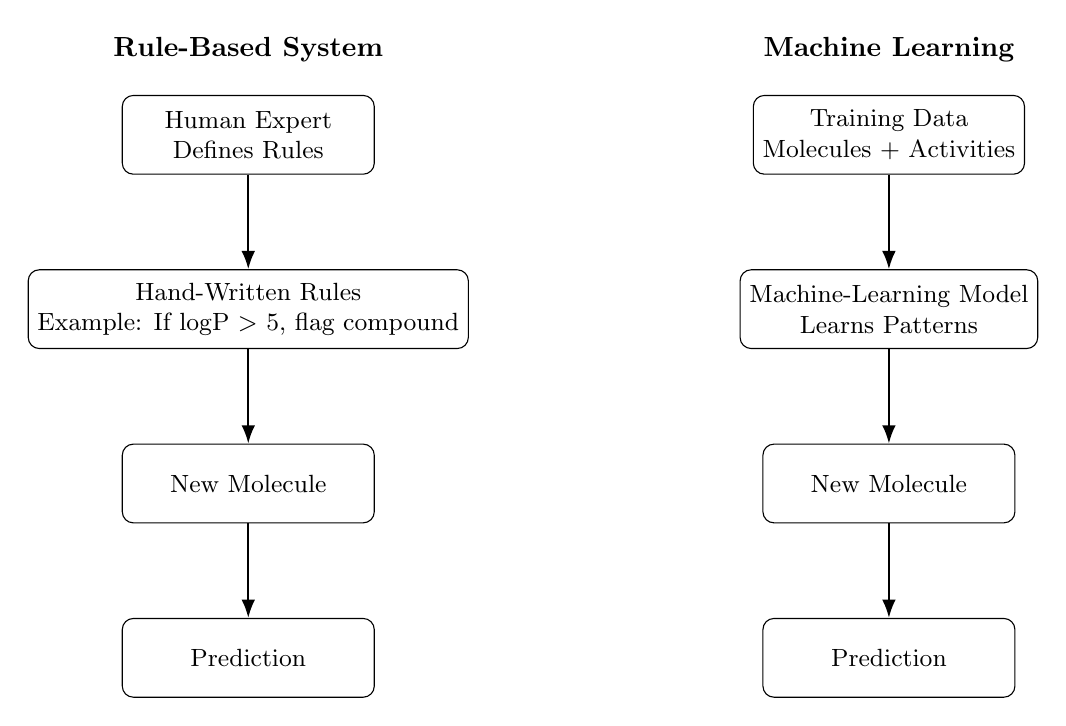
\begin{tikzpicture}[
    node distance=1.2cm,
    box/.style={
        rectangle,
        draw,
        rounded corners,
        align=center,
        minimum width=3.2cm,
        minimum height=1cm,
        font=\small
    },
    arrow/.style={-{Latex}, thick}
]

% Rule-based side
\node[box] (expert) {Human Expert\\Defines Rules};
\node[box, below=of expert] (rules) {Hand-Written Rules\\Example: If logP $>$ 5, flag compound};
\node[box, below=of rules] (ruleinput) {New Molecule};
\node[box, below=of ruleinput] (ruleoutput) {Prediction};

\draw[arrow] (expert) -- (rules);
\draw[arrow] (rules) -- (ruleinput);
\draw[arrow] (ruleinput) -- (ruleoutput);

\node[above=0.3cm of expert, font=\bfseries] {Rule-Based System};

% ML side
\node[box, right=4.8cm of expert] (data) {Training Data\\Molecules + Activities};
\node[box, below=of data] (mlmodel) {Machine-Learning Model\\Learns Patterns};
\node[box, below=of mlmodel] (mlinput) {New Molecule};
\node[box, below=of mlinput] (mloutput) {Prediction};

\draw[arrow] (data) -- (mlmodel);
\draw[arrow] (mlmodel) -- (mlinput);
\draw[arrow] (mlinput) -- (mloutput);

\node[above=0.3cm of data, font=\bfseries] {Machine Learning};

\end{tikzpicture}
\caption{Comparison between a rule-based system and a machine-learning system. In a rule-based system, an expert manually defines the rules. In machine learning, the model learns patterns from examples in the training data.}
\label{fig:rule-based-vs-ml}
\end{figure}

The key difference is:

\begin{center}
\textbf{Rule-based system: Human defines the rules.}

\textbf{Machine learning: The model learns the rules from data.}
\end{center}

\subsection*{Why Machine Learning Is Useful in QSAR}

In QSAR, chemical activity can depend on many molecular properties at the same time. These relationships may be complex and difficult to describe using simple human-written rules.

Machine learning is useful because it can learn relationships involving many descriptors simultaneously. For example, a model may learn that toxicity depends on a combination of molecular size, hydrophobicity, polarity, electronic effects, and specific structural fragments.

\begin{instructornote}
A useful explanation for students is that machine learning does not replace chemical knowledge. Instead, it helps detect patterns that may be difficult to manually define, and the researcher still needs to interpret whether those patterns make chemical sense.
\end{instructornote}

% ------------------------------------------------------------
\section{Regression vs. Classification}

QSAR models are usually divided into two main types: \textbf{regression models} and \textbf{classification models}.

\subsection{Regression}

A \textbf{regression model} predicts a continuous numerical value.

Examples of regression endpoints include:

\begin{itemize}[leftmargin=*]
    \item LD$_{50}$,
    \item IC$_{50}$,
    \item EC$_{50}$,
    \item solubility,
    \item boiling point,
    \item melting point,
    \item binding affinity.
\end{itemize}

For example, if the goal is to predict the exact toxicity value of a compound, this is a regression problem.

\[
\text{Molecule} \rightarrow \text{Model} \rightarrow \text{Predicted LD}_{50}
\]

\subsection{Classification}

A \textbf{classification model} predicts a category or class label.

Examples of classification endpoints include:

\begin{itemize}[leftmargin=*]
    \item toxic vs. non-toxic,
    \item active vs. inactive,
    \item inhibitor vs. non-inhibitor,
    \item soluble vs. poorly soluble,
    \item mutagenic vs. non-mutagenic.
\end{itemize}

For example, if the goal is to classify whether a compound is toxic or non-toxic, this is a classification problem.

\[
\text{Molecule} \rightarrow \text{Model} \rightarrow \text{Toxic or Non-Toxic}
\]

\subsection*{Regression and Classification Examples}

\begin{center}
\begin{tabular}{lll}
\toprule
\textbf{QSAR Task} & \textbf{Output Type} & \textbf{Model Type} \\
\midrule
Predict LD$_{50}$ value & Continuous number & Regression \\
Predict IC$_{50}$ value & Continuous number & Regression \\
Predict solubility & Continuous number & Regression \\
Predict toxic vs. non-toxic & Category & Classification \\
Predict active vs. inactive & Category & Classification \\
Predict inhibitor vs. non-inhibitor & Category & Classification \\
\bottomrule
\end{tabular}
\end{center}

\begin{exercise}
For each endpoint below, ask the student to decide whether the problem is regression or classification:

\begin{enumerate}[leftmargin=*]
    \item Predicting the exact IC$_{50}$ value of a compound.
    \item Predicting whether a compound is active or inactive.
    \item Predicting the aqueous solubility of a molecule.
    \item Predicting whether a compound is mutagenic or non-mutagenic.
    \item Predicting the LD$_{50}$ value of a chemical.
\end{enumerate}
\end{exercise}

% ------------------------------------------------------------
\section{Overfitting and Underfitting}

When building a QSAR model, the goal is not just to fit the training data well. The goal is to build a model that can make reliable predictions for new compounds.

Two common modeling problems are \textbf{overfitting} and \textbf{underfitting}.

\subsection{Underfitting}

\textbf{Underfitting} occurs when the model is too simple to learn the relationship between molecular descriptors and the endpoint.

An underfit model performs poorly on both the training set and the test set.

For example, a simple linear regression model may underfit if the true relationship between descriptors and toxicity is highly nonlinear.

\subsection{Overfitting}

\textbf{Overfitting} occurs when the model learns the training data too well, including noise or random patterns that are not meaningful.

An overfit model usually performs very well on the training set but poorly on the test set.

This is especially important in QSAR because datasets are often small, while the number of descriptors can be very large. For example, a dataset may contain only 100 molecules but thousands of descriptors. In this situation, a model may easily memorize the training compounds instead of learning general chemical patterns.

\begin{figure}[h]
    \centering
    \includegraphics[width=0.85\textwidth]{figures/overfit_vs_underfit.jpg}
    \caption{Underfitting vs. overfitting. A good fit finds the general trend of data and will give the most reliable prediction for an unseen datapoint. }
    \label{fig:fitting}
\end{figure}


\subsection{Good Generalization}

A good QSAR model should have reasonable performance on both the training set and the test set. The test-set performance is especially important because it estimates how well the model may perform on new molecules.

\begin{center}
\begin{tabular}{llll}
\toprule
\textbf{Situation} & \textbf{Training Performance} & \textbf{Test Performance} & \textbf{Interpretation} \\
\midrule
Underfitting & Poor & Poor & Model is too simple \\
Overfitting & Very good & Poor & Model memorized training data \\
Good fit & Good & Good & Model generalizes better \\
\bottomrule
\end{tabular}
\end{center}

\begin{instructornote}
A simple analogy is exam preparation. Underfitting is like not studying enough. Overfitting is like memorizing answers to practice questions without understanding the subject. A good model is like a student who understands the material and can answer new questions.
\end{instructornote}

% ------------------------------------------------------------
\section{Feature Selection}

Feature selection is the process of selecting a smaller set of useful descriptors from a larger descriptor pool.

In QSAR, feature selection is important because descriptor datasets can be very large. A single molecule may have hundreds or thousands of calculated descriptors. However, not all descriptors are useful for predicting the endpoint.

Some descriptors may be:

\begin{itemize}[leftmargin=*]
    \item irrelevant to the endpoint,
    \item redundant with other descriptors,
    \item noisy,
    \item difficult to interpret,
    \item harmful to model generalization.
\end{itemize}

Using too many descriptors can increase the risk of overfitting, especially when the dataset is small.

\subsection{Why Feature Selection Is Important}

Feature selection can help:

\begin{itemize}[leftmargin=*]
    \item reduce overfitting,
    \item improve model performance on external test sets,
    \item reduce model complexity,
    \item make models easier to interpret,
    \item remove redundant or noisy descriptors,
    \item decrease computational cost.
\end{itemize}

For example, if a QSAR dataset contains 150 molecules and 2,000 descriptors, the model has many more features than compounds. Without feature selection, the model may find random patterns that do not generalize to new molecules.

\begin{center}
\[
\text{Large descriptor pool} \rightarrow \text{Feature selection} \rightarrow \text{Smaller useful descriptor set}
\]
\end{center}

\subsection{Sequential Feature Selection}

\textbf{Sequential feature selection} is a step-by-step method for selecting descriptors.

There are two common types:

\begin{itemize}[leftmargin=*]
    \item \textbf{Forward selection:} starts with no descriptors and adds one descriptor at a time.
    \item \textbf{Backward selection:} starts with all descriptors and removes one descriptor at a time.
\end{itemize}

In forward selection, the algorithm tests which descriptor improves the model the most and adds it to the selected set. Then it repeats the process by adding another descriptor. This continues until a stopping condition is reached, such as a selected number of descriptors or no further improvement in validation performance.

\subsubsection*{Forward Sequential Feature Selection Workflow}

\begin{enumerate}[leftmargin=*]
    \item Start with an empty descriptor set.
    \item Train models using each candidate descriptor.
    \item Select the descriptor that gives the best validation performance.
    \item Add that descriptor to the selected set.
    \item Repeat the process by testing the remaining descriptors.
    \item Stop when the desired number of descriptors is selected or performance no longer improves.
\end{enumerate}

\begin{lstlisting}[style=pythonstyle, caption={Example of sequential feature selection using scikit-learn.}]
from sklearn.feature_selection import SequentialFeatureSelector
from sklearn.ensemble import RandomForestRegressor
from sklearn.model_selection import KFold

# Define the model
model = RandomForestRegressor(
    n_estimators=300,
    random_state=42
)

# Define cross-validation
cv = KFold(
    n_splits=5,
    shuffle=True,
    random_state=42
)

# Sequential feature selection
sfs = SequentialFeatureSelector(
    estimator=model,
    n_features_to_select=10,
    direction="forward",
    scoring="r2",
    cv=cv,
    n_jobs=-1
)

# Fit feature selector using training data only
sfs.fit(X_train, y_train)

# Selected descriptor names
selected_features = X_train.columns[sfs.get_support()]

print("Selected descriptors:")
print(selected_features.tolist())

# Create reduced train and test sets using the same selected descriptors
X_train_selected = X_train[selected_features]
X_test_selected = X_test[selected_features]
\end{lstlisting}

\textbf{Important:} Feature selection should be performed using only the training set. After the descriptors are selected from the training set, the same descriptors should be selected from the test set. The test set should not be used during feature selection.

\subsection{Genetic Algorithm-Based Feature Selection}

A \textbf{genetic algorithm}, often abbreviated as GA, is an optimization method inspired by natural selection. In QSAR, a genetic algorithm can be used to search for a good subset of descriptors.

Instead of adding or removing descriptors one at a time, a genetic algorithm starts with many possible descriptor subsets. Each subset is evaluated using model performance. The best subsets are selected, modified, and combined to produce new subsets.

\subsubsection*{Basic Genetic Algorithm Concepts}

\begin{center}
\begin{tabular}{ll}
\toprule
\textbf{GA Term} & \textbf{Meaning in Feature Selection} \\
\midrule
Individual & One possible descriptor subset \\
Population & A group of descriptor subsets \\
Fitness & Model performance for a descriptor subset \\
Selection & Choosing better-performing subsets \\
Crossover & Combining parts of two descriptor subsets \\
Mutation & Randomly adding or removing descriptors \\
Generation & One cycle of selection, crossover, and mutation \\
\bottomrule
\end{tabular}
\end{center}

\subsubsection*{Genetic Algorithm Workflow}

\begin{enumerate}[leftmargin=*]
    \item Generate an initial population of random descriptor subsets.
    \item Train and validate a model for each subset.
    \item Assign a fitness score to each subset based on model performance.
    \item Select the better-performing subsets.
    \item Create new subsets using crossover and mutation.
    \item Repeat the process for multiple generations.
    \item Choose the descriptor subset with the best validation performance.
\end{enumerate}

A simple way to think about GA feature selection is:

\[
\text{Many possible descriptor subsets} \rightarrow \text{Evolutionary search} \rightarrow \text{Best descriptor subset}
\]

\subsubsection*{Why Use a Genetic Algorithm?}

Genetic algorithms can be useful when the descriptor space is large and many descriptor combinations are possible. They are able to search a wider range of possible feature subsets compared with simple sequential methods.

However, genetic algorithms can also be computationally expensive because many models must be trained during the search. The results may also depend on settings such as population size, mutation rate, crossover rate, and number of generations.

\subsection{Sequential Feature Selection vs. Genetic Algorithm}

\begin{center}
\begin{tabular}{p{0.25\textwidth}p{0.32\textwidth}p{0.32\textwidth}}
\toprule
\textbf{Method} & \textbf{Advantages} & \textbf{Limitations} \\
\midrule
Sequential Feature Selection & Easy to understand; systematic; available in scikit-learn & Can be slow; may miss better descriptor combinations \\
Genetic Algorithm & Searches many possible combinations; useful for large descriptor spaces & More complex; computationally expensive; requires parameter tuning \\
\bottomrule
\end{tabular}
\end{center}


% ------------------------------------------------------------
\section{Summary}

Machine learning models learn relationships between molecular descriptors and experimental endpoints. Unlike rule-based systems, where an expert manually defines the rules, machine-learning models learn patterns from examples in the training data.

QSAR problems can be regression problems, where the goal is to predict a continuous value, or classification problems, where the goal is to predict a category. Model performance must be evaluated carefully to avoid underfitting and overfitting.

Feature selection is an important step in QSAR because molecular descriptor datasets often contain many irrelevant or redundant descriptors. Methods such as sequential feature selection and genetic algorithms can help identify smaller and more useful descriptor subsets.

\begin{exercise}
Ask the student to answer the following questions:

\begin{enumerate}[leftmargin=*]
    \item What is the main difference between a rule-based system and a machine-learning model?
    \item Is predicting IC$_{50}$ a regression or classification problem?
    \item Is predicting active vs. inactive a regression or classification problem?
    \item What is overfitting?
    \item Why can too many descriptors be a problem in QSAR?
    \item What is the difference between sequential feature selection and genetic algorithm-based feature selection?
\end{enumerate}
\end{exercise}


% ============================================================
% ============================================================
\chapter{Internal and External Validation}

\begin{learningobjectives}
    \item Understand the difference between internal and external validation.
    \item Explain why validation is necessary in QSAR modeling.
    \item Understand k-fold cross-validation 
    \item Understand leave-one-out cross-validation.
    \item Explain the role of an external test set in evaluating QSAR models.
\end{learningobjectives}

Validation is one of the most important parts of QSAR modeling. A model should not only fit the training data well; it should also make reliable predictions for new molecules. Validation methods help estimate how well a model may perform when applied to compounds that were not used to build it.

In QSAR, validation is often divided into two major categories:

\begin{itemize}[leftmargin=*]
    \item \textbf{Internal validation:} model performance is evaluated using only the training data, usually through resampling methods such as cross-validation.
    \item \textbf{External validation:} model performance is evaluated using an independent test set that was not used during model training.
\end{itemize}

Both types of validation are important. Internal validation helps assess the stability of the model during development, while external validation provides a more realistic estimate of prediction performance on new compounds.

% ------------------------------------------------------------
\section{Internal Validation}

\textbf{Internal validation} refers to validation methods performed within the training dataset. The goal is to estimate how stable and reliable the model is without using the external test set.

Internal validation is useful because one train/test split may not be enough to fully evaluate a model. Depending on how the data are split, the model may appear better or worse. Cross-validation helps reduce this problem by repeatedly training and validating the model on different subsets of the training data.

Common internal validation methods include:

\begin{itemize}[leftmargin=*]
    \item k-fold cross-validation,
    \item leave-one-out cross-validation.
\end{itemize}

\textbf{Important:} Internal validation should be performed using only the training set. The external test set should remain untouched until final model evaluation.

% ------------------------------------------------------------
\subsection{K-Fold Cross-Validation}

In \textbf{k-fold cross-validation}, the training data are divided into $k$ approximately equal parts, called folds. The model is trained using $k-1$ folds and validated on the remaining fold. This process is repeated $k$ times so that each fold is used once as the validation fold.

For example, in \textbf{5-fold cross-validation}, the training data are divided into five folds:

\[
\text{Fold 1, Fold 2, Fold 3, Fold 4, Fold 5}
\]

The model is trained and validated five times:

\begin{center}
\begin{tabular}{lll}
\toprule
\textbf{Round} & \textbf{Training Folds} & \textbf{Validation Fold} \\
\midrule
1 & Folds 2, 3, 4, 5 & Fold 1 \\
2 & Folds 1, 3, 4, 5 & Fold 2 \\
3 & Folds 1, 2, 4, 5 & Fold 3 \\
4 & Folds 1, 2, 3, 5 & Fold 4 \\
5 & Folds 1, 2, 3, 4 & Fold 5 \\
\bottomrule
\end{tabular}
\end{center}

After the five rounds are complete, the validation scores are averaged. This average cross-validation score gives an estimate of how well the model performs across different subsets of the training data.

\[
\text{Mean CV score} =
\frac{\text{Score}_1 + \text{Score}_2 + \text{Score}_3 + \text{Score}_4 + \text{Score}_5}{5}
\]

\begin{figure}[htbp]
    \centering
    \includegraphics[width=0.7\textwidth]{figures/cross_validation.jpg}
    \caption{visualization of 5-fold cross-validation. Remember that this is an internal validation technique, meaning that we split the training data into 5 folds, we train the model on 4 folds, and we test on the fold we skip, then we repeat the process 5 times so that we have each fold as a test set. Once we make sure the model shows a good performance and stabilization over different folds, we can use it to predict the unseen test set.}
    \label{fig:crossvalidation}
\end{figure}


For regression QSAR models, the score may be $R^2$, MAE, or RMSE. For classification QSAR models, the score may be accuracy, F1-score, MCC, or ROC-AUC.

\begin{lstlisting}[style=pythonstyle, caption={Example of 5-fold cross-validation for a regression QSAR model.}]
from sklearn.model_selection import KFold, cross_val_score
from sklearn.ensemble import RandomForestRegressor
import numpy as np

# Define the model
model = RandomForestRegressor(
    n_estimators=300,
    random_state=42
)

# Define 5-fold cross-validation
cv = KFold(
    n_splits=5,
    shuffle=True,
    random_state=42
)

# Perform cross-validation using training data only
cv_scores = cross_val_score(
    model,
    X_train,
    y_train,
    cv=cv,
    scoring="r2"
)

print("5-fold CV R2 scores:", cv_scores)
print("Mean CV R2:", np.mean(cv_scores))
print("Standard deviation:", np.std(cv_scores))
\end{lstlisting}

The mean cross-validation score shows the average internal performance of the model. The standard deviation shows how much the performance changes across different folds. A large standard deviation may suggest that the model is unstable or that the dataset is small or heterogeneous.

% ------------------------------------------------------------
\subsection{Leave-One-Out Cross-Validation}

\textbf{Leave-one-out cross-validation}, often abbreviated as LOOCV, is a special case of k-fold cross-validation where the number of folds is equal to the number of training samples.

In LOOCV, one compound is left out as the validation sample, and the model is trained on all remaining compounds. This process is repeated until every compound has been used once as the validation sample.

If the training set contains $n$ compounds, LOOCV trains the model $n$ times.

For example, if a training set contains 100 compounds:

\[
k = n = 100
\]

This means the model is trained 100 times. Each time, 99 compounds are used for training and 1 compound is used for validation.

\begin{center}
\begin{tabular}{lll}
\toprule
\textbf{Round} & \textbf{Training Set} & \textbf{Validation Compound} \\
\midrule
1 & All compounds except compound 1 & Compound 1 \\
2 & All compounds except compound 2 & Compound 2 \\
3 & All compounds except compound 3 & Compound 3 \\
$\cdots$ & $\cdots$ & $\cdots$ \\
$n$ & All compounds except compound $n$ & Compound $n$ \\
\bottomrule
\end{tabular}
\end{center}

LOOCV can be useful for small datasets because it uses almost all available data for training in each round. However, it can be computationally expensive for large datasets because the model must be trained many times.

\begin{lstlisting}[style=pythonstyle, caption={Example of leave-one-out cross-validation.}]
from sklearn.model_selection import LeaveOneOut, cross_val_score
from sklearn.ensemble import RandomForestRegressor
import numpy as np

# Define the model
model = RandomForestRegressor(
    n_estimators=300,
    random_state=42
)

# Define leave-one-out cross-validation
loo = LeaveOneOut()

# Perform LOOCV using training data only
loo_scores = cross_val_score(
    model,
    X_train,
    y_train,
    cv=loo,
    scoring="r2"
)

print("Number of LOOCV rounds:", len(loo_scores))
print("Mean LOOCV R2:", np.mean(loo_scores))
\end{lstlisting}

\textbf{Note:} In practice, $R^2$ may not always be meaningful for a single validation sample in each LOOCV round. Therefore, for regression tasks, it is often better to collect all LOOCV predictions and then calculate overall metrics such as $R^2$, MAE, and RMSE.

\begin{lstlisting}[style=pythonstyle, caption={LOOCV predictions followed by overall regression metrics.}]
from sklearn.model_selection import LeaveOneOut, cross_val_predict
from sklearn.ensemble import RandomForestRegressor
from sklearn.metrics import r2_score, mean_absolute_error, mean_squared_error
import numpy as np

model = RandomForestRegressor(
    n_estimators=300,
    random_state=42
)

loo = LeaveOneOut()

# Generate cross-validated predictions
y_pred_loo = cross_val_predict(
    model,
    X_train,
    y_train,
    cv=loo
)

# Calculate overall LOOCV metrics
r2_loo = r2_score(y_train, y_pred_loo)
mae_loo = mean_absolute_error(y_train, y_pred_loo)
rmse_loo = np.sqrt(mean_squared_error(y_train, y_pred_loo))

print("LOOCV R2:", r2_loo)
print("LOOCV MAE:", mae_loo)
print("LOOCV RMSE:", rmse_loo)
\end{lstlisting}

\subsection{Internal Validation Summary}

Internal validation helps answer the question:

\begin{quote}
How stable is the model during training?
\end{quote}

However, internal validation is not a replacement for external validation. Even if a model performs well during cross-validation, it still needs to be evaluated on an independent external test set.

% ------------------------------------------------------------
\section{External Validation}

\textbf{External validation} evaluates the final model using a separate test set that was not used during model training or model selection.

The external test set should not be used for:

\begin{itemize}[leftmargin=*]
    \item descriptor filtering,
    \item feature selection,
    \item hyperparameter tuning,
    \item model comparison,
    \item scaling parameter estimation,
    \item cross-validation.
\end{itemize}

The purpose of external validation is to estimate how well the model performs on new compounds. In QSAR, this is especially important because the final goal is usually to predict activities for molecules that have not yet been experimentally tested.

\subsection{External Test Set Workflow}

A proper external validation workflow is:

\begin{enumerate}[leftmargin=*]
    \item Split the dataset into training and external test sets.
    \item Use only the training set for preprocessing decisions, feature selection, model training, cross-validation, and hyperparameter tuning.
    \item Train the final model using the selected training data and selected descriptors.
    \item Apply the same preprocessing steps to the external test set.
    \item Predict the endpoint values for the external test set.
    \item Calculate external validation metrics.
\end{enumerate}

\begin{lstlisting}[style=pythonstyle, caption={Example of external validation after model training.}]
from sklearn.ensemble import RandomForestRegressor
from sklearn.metrics import r2_score, mean_absolute_error, mean_squared_error
import numpy as np

# Train the final model using the training set
final_model = RandomForestRegressor(
    n_estimators=300,
    random_state=42
)

final_model.fit(X_train_selected, y_train)

# Predict the external test set
y_pred_test = final_model.predict(X_test_selected)

# Calculate external validation metrics
r2_ext = r2_score(y_test, y_pred_test)
mae_ext = mean_absolute_error(y_test, y_pred_test)
rmse_ext = np.sqrt(mean_squared_error(y_test, y_pred_test))

print("External test R2:", r2_ext)
print("External test MAE:", mae_ext)
print("External test RMSE:", rmse_ext)
\end{lstlisting}

\subsection{Why External Validation Is Important}

External validation is important because it provides a more realistic estimate of model performance. A model may perform well during internal validation but still fail on truly new compounds.

This can happen when:

\begin{itemize}[leftmargin=*]
    \item the dataset is small,
    \item the model is overfit,
    \item the test compounds are chemically different from the training compounds,
    \item feature selection was not performed correctly,
    \item data leakage occurred during preprocessing,
    \item the endpoint contains experimental noise.
\end{itemize}

A strong QSAR model should show good performance in both internal and external validation.

\subsection{Internal vs. External Validation}

\begin{center}
\begin{tabular}{p{0.25\textwidth}p{0.32\textwidth}p{0.32\textwidth}}
\toprule
\textbf{Validation Type} & \textbf{Data Used} & \textbf{Purpose} \\
\midrule
Internal validation & Training data only & Estimates model stability during development \\
External validation & Independent test set & Estimates performance on new compounds \\
\bottomrule
\end{tabular}
\end{center}

\subsection{Common Mistakes}

Common validation mistakes in QSAR include:

\begin{itemize}[leftmargin=*]
    \item using the test set during feature selection,
    \item scaling the full dataset before train/test splitting,
    \item removing highly correlated descriptors using the full dataset,
    \item tuning hyperparameters based on test-set performance,
    \item reporting only training performance,
    \item reporting cross-validation performance without external validation.
\end{itemize}

These mistakes can lead to overly optimistic model performance. To avoid this, the external test set should remain independent until the final evaluation.

% ------------------------------------------------------------
\section{Summary}

Internal and external validation are both essential in QSAR modeling. Internal validation, such as 5-fold cross-validation or leave-one-out cross-validation, helps evaluate model stability during development. External validation evaluates the final model on an independent test set and provides a more realistic estimate of prediction performance.

A reliable QSAR model should not only perform well during internal validation but also show acceptable performance on external validation.

\begin{exercise}
Ask the student to answer the following questions:

\begin{enumerate}[leftmargin=*]
    \item What is the difference between internal and external validation?
    \item In 5-fold cross-validation, how many times is the model trained?
    \item In leave-one-out cross-validation, how many validation compounds are used in each round?
    \item Why should the external test set not be used during feature selection?
    \item Which validation result is more important for estimating performance on new molecules: training performance, cross-validation performance, or external test performance?
\end{enumerate}
\end{exercise}

% ============================================================
\chapter{Applicability Domain}

\begin{learningobjectives}
    \item Define applicability domain in QSAR modeling.
    \item Explain why applicability domain is important for reliable prediction.
    \item Describe common approaches for defining applicability domain.
    \item Understand distance-based, similarity-based, and Williams plot approaches.
    \item Explain the x-axis and y-axis of a Williams plot.
    \item Interpret compounds with high leverage or standardized residuals greater than $\pm 3$.
\end{learningobjectives}

A QSAR model is usually developed using a limited set of molecules. Therefore, the model is expected to make reliable predictions only for compounds that are similar to the molecules used during training. This concept is called the \textbf{applicability domain}, often abbreviated as \textbf{AD}.

% ------------------------------------------------------------
\section{What Is Applicability Domain?}

The applicability domain defines \textbf{the chemical space where a QSAR model is considered reliable}. In other words, it describes the region of chemical structures and descriptor values where the model has enough training information to make meaningful predictions.

A QSAR model should not be assumed to work equally well for every possible molecule. For example, if a model is trained only on small organic molecules, it may not make reliable predictions for very large molecules, polymers, metal complexes, or molecules with chemical features not present in the training set.

\begin{quote}
The applicability domain answers the question: \textit{Is this new molecule similar enough to the training compounds for the model prediction to be trusted?}
\end{quote}

\subsection{Why Applicability Domain Is Important}

Applicability domain is important because a model may produce a numerical prediction for any molecule, even when that prediction is not reliable. Machine-learning models usually do not automatically know when they are being applied outside their reliable chemical space.

For example, a QSAR model may predict the toxicity of a molecule that is very different from all training compounds. \textbf{The prediction may look reasonable as a number, but it may be scientifically unreliable because the model has never seen similar chemistry during training.}

Applicability domain helps identify:

\begin{itemize}[leftmargin=*]
    \item compounds that are structurally similar to the training set,
    \item compounds that are very different from the training set,
    \item predictions that may be unreliable,
    \item possible outliers in the training or test set,
    \item chemical regions where more experimental data may be needed.
\end{itemize}

In QSAR reporting, applicability domain is important because it helps prevent overinterpretation of model predictions. A good QSAR model should report not only predicted values but also whether each prediction falls inside or outside the model's applicability domain.

% ------------------------------------------------------------
\section{Approaches for Defining Applicability Domain}

Several methods can be used to define applicability domain. Different methods use different ideas of molecular similarity, descriptor space, or prediction error.

Common approaches include:

\begin{itemize}[leftmargin=*]
    \item distance-based applicability domain,
    \item similarity-based applicability domain,
    \item leverage-based applicability domain using the Williams plot.
\end{itemize}

% ------------------------------------------------------------
\subsection{Distance-Based Applicability Domain}

Distance-based methods define applicability domain based on how far a compound is from the training compounds in descriptor space.

In this approach, each molecule is represented by its molecular descriptors. A new compound is considered inside the applicability domain if it is close enough to the training compounds.

Common distance measures include:

\begin{itemize}[leftmargin=*]
    \item Euclidean distance,
    \item Mahalanobis distance,
    \item distance to nearest training compound,
    \item distance to the centroid of the training set.
\end{itemize}

For example, if a new molecule has descriptor values very far from the training molecules, it may be considered outside the applicability domain.

\[
d_i = \sqrt{(x_i - x_j)^2}
\]

where $d_i$ represents distance in descriptor space.

For multiple descriptors, Euclidean distance can be written as:

\[
d(i,j) = \sqrt{\sum_{k=1}^{p}(x_{ik} - x_{jk})^2}
\]

where:

\begin{itemize}[leftmargin=*]
    \item $x_{ik}$ is the value of descriptor $k$ for molecule $i$,
    \item $x_{jk}$ is the value of descriptor $k$ for molecule $j$,
    \item $p$ is the number of descriptors.
\end{itemize}

\subsubsection*{Interpretation}

A molecule close to the training compounds is more likely to be inside the applicability domain. A molecule far from the training compounds may be outside the applicability domain and its prediction should be treated with caution.

\begin{center}
\begin{tabular}{ll}
\toprule
\textbf{Distance Result} & \textbf{Interpretation} \\
\midrule
Small distance to training compounds & More likely inside AD \\
Large distance to training compounds & More likely outside AD \\
\bottomrule
\end{tabular}
\end{center}

% ------------------------------------------------------------
\subsection{Similarity-Based Applicability Domain}

Similarity-based methods define applicability domain based on molecular similarity to the training set. These methods are commonly used when molecules are represented by fingerprints, such as Morgan fingerprints.

One common similarity measure is the \textbf{Tanimoto similarity}. It is often used to compare molecular fingerprints.

Tanimoto similarity ranges from 0 to 1:

\begin{itemize}[leftmargin=*]
    \item 1 means two molecules are identical based on their fingerprints,
    \item 0 means two molecules have no fingerprint features in common.
\end{itemize}

A new molecule can be considered inside the applicability domain if it has sufficient similarity to at least one training molecule.

For example:

\[
\text{Inside AD if maximum Tanimoto similarity to training set} \geq 0.6
\]

The exact threshold depends on the dataset and the modeling task.

\subsubsection*{Interpretation}

If a test molecule is highly similar to one or more training molecules, the model is more likely to make a reliable prediction. If the molecule has low similarity to all training molecules, the prediction may be unreliable.

\begin{center}
\begin{tabular}{ll}
\toprule
\textbf{Similarity Result} & \textbf{Interpretation} \\
\midrule
High similarity to training molecules & More likely inside AD \\
Low similarity to all training molecules & More likely outside AD \\
\bottomrule
\end{tabular}
\end{center}

% ------------------------------------------------------------
\subsection{Williams Plot}

The \textbf{Williams plot} is one of the most common applicability domain methods in QSAR. It is especially common in descriptor-based QSAR modeling.

A Williams plot shows two important pieces of information:

\begin{itemize}[leftmargin=*]
    \item the \textbf{leverage} of each compound on the x-axis,
    \item the \textbf{standardized residual} of each compound on the y-axis.
\end{itemize}

The Williams plot helps identify:

\begin{itemize}[leftmargin=*]
    \item compounds that are structurally far from the training set,
    \item compounds with unusually large prediction errors,
    \item possible response outliers,
    \item compounds outside the model's applicability domain.
\end{itemize}

% ------------------------------------------------------------
\section{Understanding the Williams Plot}

\subsection{X-Axis: Leverage}

The x-axis of a Williams plot is the \textbf{leverage} value, usually written as $h_i$.

Leverage measures how far a compound is from the center of the training descriptor space. A compound with high leverage has descriptor values that are unusual compared with most training compounds.

For the training set, leverage is calculated from the hat matrix:

\[
H = X(X^TX)^{-1}X^T
\]

where:

\begin{itemize}[leftmargin=*]
    \item $H$ is the hat matrix,
    \item $X$ is the descriptor matrix,
    \item $X^T$ is the transpose of the descriptor matrix,
    \item $(X^TX)^{-1}$ is the inverse of $X^TX$.
\end{itemize}

The leverage value for compound $i$ is the $i$th diagonal element of the hat matrix:

\[
h_i = H_{ii}
\]

For a new or test compound, leverage can be calculated as:

\[
h_i = x_i^T(X^TX)^{-1}x_i
\]

where $x_i$ is the descriptor vector of the new compound.

\subsection{Warning Leverage Threshold}

A compound is usually considered to have high leverage if its leverage is greater than the warning leverage value, $h^*$.

The warning leverage is commonly calculated as:

\[
h^* = \frac{3(p+1)}{n}
\]

where:

\begin{itemize}[leftmargin=*]
    \item $p$ is the number of model descriptors,
    \item $n$ is the number of training compounds,
    \item $p+1$ includes the intercept term.
\end{itemize}

If a compound has:

\[
h_i > h^*
\]

then it is considered structurally influential or outside the main descriptor space of the training set.

\subsubsection*{Interpretation of High Leverage}

A high-leverage compound is not automatically a bad compound. It means the compound is chemically or structurally different from the majority of the training set.

For training compounds, high leverage means the compound may strongly influence the model.

For test compounds, high leverage means the compound may be outside the applicability domain, and its prediction should be interpreted carefully.

% ------------------------------------------------------------
\subsection{Y-Axis: Standardized Residual}

The y-axis of a Williams plot is the \textbf{standardized residual}.

A residual is the difference between the experimental value and the predicted value:

\[
e_i = y_i - \hat{y}_i
\]

where:

\begin{itemize}[leftmargin=*]
    \item $e_i$ is the residual for compound $i$,
    \item $y_i$ is the experimental value,
    \item $\hat{y}_i$ is the predicted value.
\end{itemize}

The standardized residual is calculated by dividing the residual by the standard deviation of residuals:

\[
r_i = \frac{e_i}{s}
\]

where:

\begin{itemize}[leftmargin=*]
    \item $r_i$ is the standardized residual,
    \item $e_i$ is the residual,
    \item $s$ is the residual standard deviation.
\end{itemize}

The residual standard deviation can be estimated from the training set as:

\[
s = \sqrt{\frac{\sum_{i=1}^{n}(y_i - \hat{y}_i)^2}{n-p-1}}
\]

where:

\begin{itemize}[leftmargin=*]
    \item $n$ is the number of training compounds,
    \item $p$ is the number of descriptors used in the model.
\end{itemize}

\subsection{Meaning of $\pm 3$ Standardized Residuals}

In a Williams plot, horizontal lines are usually drawn at:

\[
r_i = +3
\]

and

\[
r_i = -3
\]

A compound with standardized residual greater than $+3$ or less than $-3$ has a much larger prediction error than expected.

\[
|r_i| > 3
\]

This means the compound may be a \textbf{response outlier}. In other words, the compound's experimental activity is not well predicted by the model.

\subsubsection*{Interpretation of Large Standardized Residuals}

If a compound has $|r_i| > 3$, this may indicate:

\begin{itemize}[leftmargin=*]
    \item possible experimental error,
    \item unusual biological behavior,
    \item missing important descriptors,
    \item an incorrect molecular structure,
    \item a compound that follows a different mechanism of action,
    \item poor model prediction for that compound.
\end{itemize}

A large standardized residual does not automatically mean the compound should be removed. It means the compound should be investigated carefully.

% ------------------------------------------------------------
\section{Interpreting Regions of the Williams Plot}

The Williams plot can be divided into different regions based on leverage and standardized residuals.

\begin{center}
\begin{tabular}{p{0.28\textwidth}p{0.62\textwidth}}
\toprule
\textbf{Region} & \textbf{Interpretation} \\
\midrule
$h_i \leq h^*$ and $|r_i| \leq 3$ & Compound is inside the applicability domain and has acceptable prediction error. \\
$h_i > h^*$ and $|r_i| \leq 3$ & Compound has high leverage but acceptable prediction error. It may be structurally influential or outside the main chemical space. \\
$h_i \leq h^*$ and $|r_i| > 3$ & Compound has normal leverage but large prediction error. It may be a response outlier. \\
$h_i > h^*$ and $|r_i| > 3$ & Compound has high leverage and large prediction error. It is likely outside the applicability domain and should be investigated carefully. \\
\bottomrule
\end{tabular}
\end{center}

\subsection{Inside vs. Outside Applicability Domain}

A common rule is:

\begin{itemize}[leftmargin=*]
    \item A compound is considered \textbf{inside the applicability domain} if $h_i \leq h^*$ and $|r_i| \leq 3$.
    \item A compound may be considered \textbf{outside the applicability domain} if $h_i > h^*$ or $|r_i| > 3$.
\end{itemize}

However, interpretation should be done carefully. A compound with high leverage but low residual may still be predicted well. A compound with normal leverage but high residual may indicate experimental noise or missing chemical information.

% ------------------------------------------------------------
\section{Example Python Code for Williams Plot}

The following code shows how to calculate leverage, standardized residuals, and the warning leverage threshold for a regression QSAR model.

\begin{lstlisting}[style=pythonstyle, caption={Calculating leverage and standardized residuals for a Williams plot.}]
import numpy as np
import matplotlib.pyplot as plt

from sklearn.preprocessing import StandardScaler
from sklearn.ensemble import RandomForestRegressor

# X_train_selected and X_test_selected contain the selected descriptors
# y_train and y_test contain the experimental endpoint values

# Scale descriptors using training set only
scaler = StandardScaler()

X_train_scaled = scaler.fit_transform(X_train_selected)
X_test_scaled = scaler.transform(X_test_selected)

# Train a regression model
model = RandomForestRegressor(
    n_estimators=300,
    random_state=42
)

model.fit(X_train_scaled, y_train)

# Predict training and test sets
y_train_pred = model.predict(X_train_scaled)
y_test_pred = model.predict(X_test_scaled)

# Number of training compounds and number of descriptors
n_train = X_train_scaled.shape[0]
p = X_train_scaled.shape[1]

# Add intercept column for leverage calculation
X_train_aug = np.column_stack([
    np.ones(n_train),
    X_train_scaled
])

X_test_aug = np.column_stack([
    np.ones(X_test_scaled.shape[0]),
    X_test_scaled
])

# Calculate leverage values
# For training compounds
hat_matrix_train = (
    X_train_aug
    @ np.linalg.pinv(X_train_aug.T @ X_train_aug)
    @ X_train_aug.T
)

leverage_train = np.diag(hat_matrix_train)

# For test compounds
hat_matrix_test = (
    X_test_aug
    @ np.linalg.pinv(X_train_aug.T @ X_train_aug)
    @ X_test_aug.T
)

leverage_test = np.diag(hat_matrix_test)

# Calculate residuals
residuals_train = y_train - y_train_pred
residuals_test = y_test - y_test_pred

# Calculate residual standard deviation from training set
s = np.sqrt(
    np.sum(residuals_train ** 2) / (n_train - p - 1)
)

# Calculate standardized residuals
std_res_train = residuals_train / s
std_res_test = residuals_test / s

# Warning leverage threshold
h_star = 3 * (p + 1) / n_train

print("Warning leverage h*:", h_star)
\end{lstlisting}

The Williams plot can then be drawn using the leverage values on the x-axis and standardized residuals on the y-axis.

\begin{lstlisting}[style=pythonstyle, caption={Drawing a Williams plot.}]
plt.figure(figsize=(7, 5))

# Training compounds
plt.scatter(
    leverage_train,
    std_res_train,
    label="Training compounds",
    alpha=0.7
)

# Test compounds
plt.scatter(
    leverage_test,
    std_res_test,
    label="Test compounds",
    alpha=0.7
)

# Horizontal lines at standardized residuals = +3 and -3
plt.axhline(y=3, linestyle="--")
plt.axhline(y=-3, linestyle="--")

# Vertical line at warning leverage
plt.axvline(x=h_star, linestyle="--")

plt.xlabel("Leverage")
plt.ylabel("Standardized residual")
plt.title("Williams Plot")
plt.legend()
plt.show()
\end{lstlisting}

\begin{instructornote}
Although the Williams plot was originally developed for linear descriptor-based models, it is commonly used in QSAR as a practical way to evaluate chemical space and response outliers. For nonlinear models, leverage should be interpreted as a descriptor-space diagnostic rather than a complete measure of model uncertainty.
\end{instructornote}

% ------------------------------------------------------------
\section{Comparison of Applicability Domain Methods}

\begin{center}
\begin{tabular}{p{0.22\textwidth}p{0.34\textwidth}p{0.34\textwidth}}
\toprule
\textbf{AD Method} & \textbf{Main Idea} & \textbf{Useful For} \\
\midrule
Distance-based AD & Measures distance from training compounds in descriptor space & Detecting compounds far from the training descriptor distribution \\
Similarity-based AD & Measures molecular similarity to training compounds, often using fingerprints & Fingerprint-based models and structural similarity analysis \\
Williams plot & Uses leverage and standardized residuals & Identifying high-leverage compounds and response outliers \\
\bottomrule
\end{tabular}
\end{center}

% ------------------------------------------------------------
\section{Summary}

Applicability domain defines the region of chemical space where a QSAR model is expected to make reliable predictions. It is important because machine-learning models can generate predictions even for molecules that are very different from the training set.

Distance-based methods evaluate how far a compound is from the training molecules in descriptor space. Similarity-based methods evaluate how similar a compound is to the training molecules, often using molecular fingerprints. The Williams plot uses leverage and standardized residuals to identify compounds that are outside the model's descriptor space or have unusually large prediction errors.

In a Williams plot, the x-axis represents leverage, which measures how far a compound is from the training descriptor space. The y-axis represents standardized residuals, which measure prediction error. Compounds with leverage greater than the warning leverage $h^*$ may be structurally influential or outside the applicability domain. Compounds with standardized residuals greater than $\pm 3$ may be response outliers.

\begin{exercise}
Ask the student to answer the following questions:

\begin{enumerate}[leftmargin=*]
    \item What is applicability domain?
    \item Why should a QSAR prediction outside the applicability domain be treated carefully?
    \item What is the difference between distance-based and similarity-based applicability domain?
    \item What does the x-axis of a Williams plot represent?
    \item What does the y-axis of a Williams plot represent?
    \item What does it mean if a compound has leverage greater than $h^*$?
    \item What does it mean if a compound has a standardized residual greater than $+3$ or less than $-3$?
\end{enumerate}
\end{exercise}
% ============================================================
% ============================================================
\chapter{Interpreting and Explaining a QSAR Model}

\begin{learningobjectives}
    \item Explain why model interpretability is important in QSAR.
    \item Understand how molecular descriptors influence model predictions.
    \item Distinguish positive, negative, and nonlinear descriptor effects.
    \item Understand the basic idea of SHAP values.
    \item Understand the basic idea of Accumulated Local Effects.
    \item Interpret model explanations using chemical reasoning.
\end{learningobjectives}

Building a QSAR model is not only about making accurate predictions. In many scientific applications, we also want to understand \textbf{why} the model makes a prediction. This is called \textbf{model interpretation} or \textbf{model explanation}.

In QSAR modeling, interpretation is especially important because the model should help connect molecular structure to biological or physicochemical activity. A useful QSAR model should not only predict toxicity, solubility, or activity, but also provide insight into which molecular features are associated with the endpoint.

% ------------------------------------------------------------
\section{Why Interpretability Is Important}

QSAR models are often used in scientific decision-making. Therefore, it is important to understand what the model has learned from the data. If a model gives good statistical performance but cannot be explained chemically, it may be difficult to trust or use in practice.

Interpretability helps answer questions such as:

\begin{itemize}[leftmargin=*]
    \item Which descriptors are most important for prediction?
    \item Does increasing a descriptor increase or decrease the predicted endpoint?
    \item Are the relationships between descriptors and the endpoint linear or nonlinear?
    \item Are the model's learned patterns chemically reasonable?
    \item Could the model be relying on artifacts or dataset bias?
    \item Which molecular features may be responsible for high or low activity?
\end{itemize}

For example, if a toxicity model shows that increasing hydrophobicity is associated with increased toxicity, this may be chemically reasonable for some endpoints because hydrophobic compounds may interact more strongly with biological membranes. However, this relationship may not apply to every dataset or every biological system. Therefore, interpretation must always be connected to chemical and biological knowledge.

\begin{instructornote}
Emphasize to students that interpretation does not automatically prove causation. A descriptor may be important because it is statistically associated with the endpoint, but additional chemical reasoning or experimental evidence is needed before making strong mechanistic claims.
\end{instructornote}

% ------------------------------------------------------------
\section{Understanding Descriptor Effects}

In QSAR, each molecule is represented by descriptors or fingerprints. When interpreting a model, we are often interested in understanding how each descriptor affects the predicted endpoint.

For example, suppose a model predicts toxicity. We may want to know:

\begin{itemize}[leftmargin=*]
    \item Does toxicity increase as molecular weight increases?
    \item Does toxicity decrease as polarity increases?
    \item Does logP have a linear or nonlinear effect?
    \item Is there an optimal range of a descriptor where activity is highest?
    \item Are some descriptors important only for certain chemical classes?
\end{itemize}

\subsection{Positive Descriptor Effect}

A descriptor has a \textbf{positive effect} when increasing the descriptor value tends to increase the predicted endpoint.

For example, if higher MolLogP values lead to higher predicted toxicity, then MolLogP has a positive effect on the model prediction.

\[
\text{Descriptor increases} \Rightarrow \text{Predicted endpoint increases}
\]

\subsection{Negative Descriptor Effect}

A descriptor has a \textbf{negative effect} when increasing the descriptor value tends to decrease the predicted endpoint.

For example, if higher topological polar surface area, or TPSA, leads to lower predicted membrane permeability, then TPSA has a negative effect on the prediction.

\[
\text{Descriptor increases} \Rightarrow \text{Predicted endpoint decreases}
\]

\subsection{Nonlinear Descriptor Effect}

Not all descriptor effects are linear. A descriptor may have a \textbf{nonlinear effect}, meaning the relationship changes across the descriptor range.

For example, very low logP may reduce membrane interaction, moderate logP may increase biological activity, and very high logP may reduce solubility. In this case, the effect of logP is not simply positive or negative across the full range.

\[
\text{Descriptor effect may depend on descriptor range}
\]

Nonlinear relationships are common in QSAR because biological activity often depends on a balance of molecular properties such as size, hydrophobicity, polarity, charge, and shape.

\subsection{Descriptor Effects Are Model-Dependent}

Descriptor interpretation depends on the model, dataset, endpoint, and chemical space. The same descriptor may have different effects in different QSAR models.

For example, molecular weight may be positively associated with one endpoint but negatively associated with another. Therefore, descriptor effects should always be interpreted in the context of the specific dataset and endpoint.


% ------------------------------------------------------------
\section{Feature Importance}

Many machine-learning models can provide feature importance values. Feature importance gives a general ranking of descriptors based on how useful they are for prediction.

For example, a Random Forest model can estimate how much each descriptor contributes to reducing prediction error across decision trees.

\begin{lstlisting}[style=pythonstyle, caption={Extracting feature importance from a Random Forest model.}]
import pandas as pd

# model is a trained Random Forest model
# X_train_selected contains the descriptors used for training

importance_df = pd.DataFrame({
    "Descriptor": X_train_selected.columns,
    "Importance": model.feature_importances_
})

importance_df = importance_df.sort_values(
    by="Importance",
    ascending=False
)

print(importance_df.head(10))
\end{lstlisting}

Feature importance is useful as a first step, but it has limitations. It usually tells us which descriptors are important, but not exactly how they affect the prediction. For example, feature importance may show that MolLogP is important, but it does not directly tell us whether increasing MolLogP increases or decreases predicted toxicity.

To better understand descriptor effects, methods such as SHAP values and Accumulated Local Effects can be used.

% ------------------------------------------------------------
\section{SHAP Values}

SHAP stands for \textbf{SHapley Additive exPlanations}. SHAP is a model explanation method that estimates how much each descriptor contributes to a model prediction.

For a single molecule, SHAP values explain how each descriptor pushes the prediction higher or lower relative to a baseline prediction.

A simplified SHAP explanation can be written as:

\[
\hat{y}_i = \phi_0 + \sum_{j=1}^{p} \phi_{ij}
\]

where:

\begin{itemize}[leftmargin=*]
    \item $\hat{y}_i$ is the model prediction for compound $i$,
    \item $\phi_0$ is the baseline prediction,
    \item $\phi_{ij}$ is the SHAP value of descriptor $j$ for compound $i$,
    \item $p$ is the number of descriptors.
\end{itemize}

\subsection{Interpreting SHAP Values}

A SHAP value can be positive or negative.

\begin{itemize}[leftmargin=*]
    \item A \textbf{positive SHAP value} means the descriptor increases the predicted endpoint.
    \item A \textbf{negative SHAP value} means the descriptor decreases the predicted endpoint.
    \item A SHAP value close to zero means the descriptor has little effect on that specific prediction.
\end{itemize}

For example, if MolLogP has a positive SHAP value for a compound in a toxicity model, this means MolLogP pushed the prediction toward higher toxicity for that compound.


\begin{figure}[h]
    \centering
    \includegraphics[width=0.85\textwidth]{figures/SHAP_values.png}
    \caption{Example of SHAP value Beeswarm plot for a model with 7 descriptors.}
    \label{fig:SHAPvalues}
\end{figure}

In Figure 8.1, as an example in the case of SpMax\_B(P), we can see that by the value of this descriptor (blue to red color), the impact of this descriptor becomes more positive. So, lower values show a negative effect and higher values show a positive effect.


% ------------------------------------------------------------
\section{Accumulated Local Effects}

Accumulated Local Effects, often abbreviated as \textbf{ALE}, is another method for interpreting machine-learning models. ALE plots show how the model prediction changes as a descriptor changes.

ALE is useful for understanding whether a descriptor has:

\begin{itemize}[leftmargin=*]
    \item a positive relationship with the endpoint,
    \item a negative relationship with the endpoint,
    \item a nonlinear relationship with the endpoint,
    \item a threshold effect,
    \item an optimal range.
\end{itemize}

\subsection{What Does an ALE Plot Show?}

An ALE plot usually has:

\begin{itemize}[leftmargin=*]
    \item the descriptor value on the x-axis,
    \item the accumulated effect on the model prediction on the y-axis.
\end{itemize}

The x-axis shows the range of a descriptor, such as MolLogP or TPSA. The y-axis shows how the model prediction changes relative to the average effect.

\subsection{Interpreting ALE Plots}

An ALE curve can be interpreted as follows:

\begin{center}
\begin{tabular}{p{0.35\textwidth}p{0.55\textwidth}}
\toprule
\textbf{ALE Pattern} & \textbf{Interpretation} \\
\midrule
Increasing curve & Higher descriptor values increase the prediction \\
Decreasing curve & Higher descriptor values decrease the prediction \\
Flat curve & Descriptor has little effect on the prediction \\
Curved or changing slope & Descriptor has a nonlinear effect \\
Peak or valley & Descriptor may have an optimal range or threshold effect \\
\bottomrule
\end{tabular}
\end{center}


\begin{figure}[h]
    \centering
    \includegraphics[width=0.75\textwidth]{figures/ALE_plots.png}
    \caption{Example of ALE interpretation for a model with 8 descriptors (each plot is for one descriptor).}
    \label{fig:ALEplot}
\end{figure}

Figure 8.1 shows an example of ALE plots. In order to interpret the effect of each descriptor on the endpoint (toxicity in this case), we need to look at the slope of the diagram. for example in case of nHM descriptor (number of heavy atoms), the ALE plot tells us that with an increase in the nHM value (in other words, an increasing number of heavy atoms) the toxicity will decrease because the slop of the diagram is negative. 


\begin{instructornote}
Ask your student to interpret the rest of the ALE plots in Figure 8.2.
\end{instructornote}


\subsection{ALE vs. Simple Correlation}

ALE is different from simple correlation. A correlation coefficient only measures a general linear relationship between a descriptor and the endpoint. ALE uses the trained model to show how the model prediction changes across different values of a descriptor.

This is useful because many QSAR models, such as Random Forest, Gradient Boosting, XGBoost, and CatBoost, can learn nonlinear relationships.

\subsection{Example ALE Code}

The following example shows how to generate an ALE plot for one descriptor.

\begin{lstlisting}[style=pythonstyle, caption={Example of an Accumulated Local Effects plot.}]
# Install PyALE if needed:
# pip install PyALE

from PyALE import ale
import matplotlib.pyplot as plt

# model is a trained regression model
# X_train_selected contains the descriptors used for training

descriptor_name = "MolLogP"

ale_eff = ale(
    X=X_train_selected,
    model=model,
    feature=[descriptor_name],
    grid_size=20
)

plt.title("ALE Plot for " + descriptor_name)
plt.xlabel(descriptor_name)
plt.ylabel("Accumulated local effect")
plt.show()
\end{lstlisting}

\subsection{Using ALE for QSAR Interpretation}

In QSAR, ALE plots can help identify descriptor--endpoint relationships. For example:

\begin{itemize}[leftmargin=*]
    \item An increasing ALE curve for MolLogP may suggest that hydrophobicity increases the predicted endpoint.
    \item A decreasing ALE curve for TPSA may suggest that polarity decreases the predicted endpoint.
    \item A nonlinear ALE curve for molecular weight may suggest that activity increases only within a certain molecular-size range.
\end{itemize}

These trends should be interpreted chemically and compared with known mechanisms, literature, or experimental observations.

% ------------------------------------------------------------


% ------------------------------------------------------------
\section{Important Cautions}

Model interpretation should be done carefully. A model explanation shows what the model has learned from the dataset, but it does not automatically prove a chemical mechanism.

Important cautions include:

\begin{itemize}[leftmargin=*]
    \item Descriptor importance does not prove causation.
    \item Correlated descriptors can make interpretation more difficult.
    \item A descriptor may be important because it is correlated with another chemical property.
    \item Interpretation is only meaningful within the model's applicability domain.
    \item Poor-quality data can lead to misleading explanations.
    \item Chemical reasoning is still necessary.
\end{itemize}

For example, if a model identifies molecular weight as important, this does not necessarily mean molecular weight itself causes toxicity. Molecular weight may be correlated with hydrophobicity, size, number of atoms, or other structural properties.

% ------------------------------------------------------------
\section{Summary}

Interpreting and explaining a QSAR model helps connect machine-learning predictions to chemical understanding. Interpretability is important because QSAR models are often used for scientific reasoning, compound prioritization, and hypothesis generation.

In QSAR interpretation, we are often interested in how each descriptor affects the predicted endpoint. A descriptor may increase the prediction, decrease the prediction, or show a nonlinear relationship with the endpoint.

SHAP values explain how descriptors contribute to model predictions. They can be used for both global interpretation across the dataset and local interpretation for individual molecules. Accumulated Local Effects plots show how model predictions change as a descriptor value changes, making them useful for identifying positive, negative, and nonlinear descriptor effects.

A reliable interpretation should combine statistical explanation methods with chemical knowledge.

% ============================================================
\appendix

\chapter{Example Dataset Template (To be updated/placeholder)}

A simple CSV file for the tutorial can use the following format:

\begin{center}
\begin{tabular}{lll}
\toprule
\textbf{CompoundID} & \textbf{SMILES} & \textbf{Activity} \\
\midrule
Cmpd001 & CCO & 1.25 \\
Cmpd002 & CC(=O)O & 0.95 \\
Cmpd003 & c1ccccc1 & 2.80 \\
\bottomrule
\end{tabular}
\end{center}

\chapter{Suggested Student Report Template}

\section*{Title}

A short title describing the QSAR task.

\section*{Introduction}

What endpoint was predicted and why is it important?

\section*{Dataset}

Where did the data come from? How many compounds were used? What cleaning steps were performed?

\section*{Methods}

What descriptors or fingerprints were calculated? What models were trained? How was validation performed?

\section*{Results}

Include a model performance table and predicted vs. experimental plot.

\section*{Discussion}

Which model performed best? Was there evidence of overfitting? Which descriptors were important? Are the results chemically meaningful?

\section*{Limitations}

Describe limitations such as dataset size, endpoint variability, applicability domain, or lack of external validation.

\section*{Conclusion}

Summarize the main result in two or three sentences.

\chapter{Useful Resources}

\begin{itemize}[leftmargin=*]
    \item RDKit documentation: \url{https://www.rdkit.org/docs/}
    \item scikit-learn documentation: \url{https://scikit-learn.org/stable/}
    \item pandas documentation: \url{https://pandas.pydata.org/docs/}
    \item DeepChem tutorials: \url{https://deepchem.io/}
\end{itemize}






\end{document}
